\documentclass[11pt]{article}
\usepackage[preprint,hyperref]{acl}
\usepackage[T1]{fontenc}
\usepackage{times,latexsym,booktabs,graphicx,amsmath,amssymb,url,placeins}
\DeclareRobustCommand{\claim}[2]{#2}
\newcommand{\RNResource}{501}
\newcommand{\RNCore}{138}
\newcommand{\RNPrimary}{76}
\newcommand{\RNFact}{45}
\newcommand{\RNDependency}{45}
\newcommand{\RNSource}{44}
\newcommand{\RNInstrument}{12}
\newcommand{\RNARRCore}{60}
\newcommand{\RNARRUnique}{423}
\newcommand{\RNAliases}{49}
\newcommand{\RNCoreAliases}{22}
\newcommand{\RNModelPairs}{720}
\newcommand{\RNAudit}{552}
\newcommand{\RNForms}{1104}
\newcommand{\RNAdj}{85}
\newcommand{\RNPositive}{11}
\newcommand{\RBroadBM}{33.9}
\newcommand{\RBroadRoute}{45.8}
\newcommand{\RBroadGain}{11.9}
\newcommand{\RBroadGroupGain}{11.6}
\newcommand{\RBroadLow}{-0.7}
\newcommand{\RBroadHigh}{30.5}
\newcommand{\RFiveClosed}{31.7}
\newcommand{\RFiveBM}{31.3}
\newcommand{\RFiveGold}{49.0}
\newcommand{\RBMHit}{53.3}
\newcommand{\RBMWrong}{60.0}
\newcommand{\RRouteHit}{98.3}
\newcommand{\RRouteWrong}{6.7}
\newcommand{\ROCCorrect}{63.0}
\newcommand{\ROCFull}{64.5}
\newcommand{\ROCFidelity}{74.6}
\newcommand{\ROCValue}{86.6}
\newcommand{\ROCQual}{76.0}
\newcommand{\ROCGroupCorrect}{67.0}
\newcommand{\ROCUnsupported}{5}
\newcommand{\RODCorrect}{71.7}
\newcommand{\RODFull}{77.5}
\newcommand{\RODFidelity}{81.2}
\newcommand{\RODValue}{96.6}
\newcommand{\RODQual}{84.2}
\newcommand{\RODGroupCorrect}{67.0}
\newcommand{\RODUnsupported}{8}
\newcommand{\RQCCorrect}{60.9}
\newcommand{\RQCFull}{70.3}
\newcommand{\RQCFidelity}{65.9}
\newcommand{\RQCValue}{89.7}
\newcommand{\RQCQual}{75.2}
\newcommand{\RQCGroupCorrect}{62.7}
\newcommand{\RQCUnsupported}{20}
\newcommand{\RQDCorrect}{83.3}
\newcommand{\RQDFull}{92.0}
\newcommand{\RQDFidelity}{81.9}
\newcommand{\RQDValue}{98.7}
\newcommand{\RQDQual}{96.8}
\newcommand{\RQDGroupCorrect}{77.3}
\newcommand{\RQDUnsupported}{17}
\newcommand{\RAgreeCorrect}{92.4}
\newcommand{\RKappaCorrect}{0.837}
\newcommand{\RAgreeFidelity}{96.0}
\newcommand{\RKappaFidelity}{0.891}
\newcommand{\RAgreeAtom}{97.8}
\newcommand{\RKappaAtom}{0.894}

\renewcommand{\RNModelPairs}{840}
\renewcommand{\RNPositive}{13}
\renewcommand{\RBroadBM}{35.7}
\renewcommand{\RBroadRoute}{47.4}
\renewcommand{\RBroadGain}{11.7}
\renewcommand{\RBroadGroupGain}{11.4}
\renewcommand{\RBroadLow}{-3.4}
\renewcommand{\RBroadHigh}{32.8}
\renewcommand{\RFiveClosed}{34.0}
\renewcommand{\RFiveBM}{34.8}
\renewcommand{\RFiveGold}{54.5}
\newcommand{\RRoutingWins}{156}
\newcommand{\RRoutingTies}{626}
\newcommand{\RRoutingLosses}{58}
\newcommand{\RSliceHitClosed}{50.0}
\newcommand{\RSliceHitBM}{65.2}
\newcommand{\RSliceHitGold}{71.0}
\newcommand{\RSliceMissClosed}{15.8}
\newcommand{\RSliceMissBM}{0.0}
\newcommand{\RSliceMissGold}{35.7}

\providecommand{\RNAudit}{}\renewcommand{\RNAudit}{1104}
\providecommand{\RNForms}{}\renewcommand{\RNForms}{2208}
\providecommand{\RNAdj}{}\renewcommand{\RNAdj}{113}
\providecommand{\ROCCorrect}{}\renewcommand{\ROCCorrect}{63.0}
\providecommand{\ROCValue}{}\renewcommand{\ROCValue}{86.6}
\providecommand{\ROCQual}{}\renewcommand{\ROCQual}{76.0}
\providecommand{\ROCFull}{}\renewcommand{\ROCFull}{64.5}
\providecommand{\ROCFidelity}{}\renewcommand{\ROCFidelity}{74.6}
\providecommand{\ROCGroupCorrect}{}\renewcommand{\ROCGroupCorrect}{67.0}
\providecommand{\ROCUnsupported}{}\renewcommand{\ROCUnsupported}{5}
\providecommand{\RODCorrect}{}\renewcommand{\RODCorrect}{71.7}
\providecommand{\RODValue}{}\renewcommand{\RODValue}{96.6}
\providecommand{\RODQual}{}\renewcommand{\RODQual}{84.2}
\providecommand{\RODFull}{}\renewcommand{\RODFull}{77.5}
\providecommand{\RODFidelity}{}\renewcommand{\RODFidelity}{81.2}
\providecommand{\RODGroupCorrect}{}\renewcommand{\RODGroupCorrect}{67.0}
\providecommand{\RODUnsupported}{}\renewcommand{\RODUnsupported}{8}
\providecommand{\RQCCorrect}{}\renewcommand{\RQCCorrect}{60.9}
\providecommand{\RQCValue}{}\renewcommand{\RQCValue}{89.7}
\providecommand{\RQCQual}{}\renewcommand{\RQCQual}{75.2}
\providecommand{\RQCFull}{}\renewcommand{\RQCFull}{70.3}
\providecommand{\RQCFidelity}{}\renewcommand{\RQCFidelity}{65.9}
\providecommand{\RQCGroupCorrect}{}\renewcommand{\RQCGroupCorrect}{62.7}
\providecommand{\RQCUnsupported}{}\renewcommand{\RQCUnsupported}{20}
\providecommand{\RQDCorrect}{}\renewcommand{\RQDCorrect}{83.3}
\providecommand{\RQDValue}{}\renewcommand{\RQDValue}{98.7}
\providecommand{\RQDQual}{}\renewcommand{\RQDQual}{96.8}
\providecommand{\RQDFull}{}\renewcommand{\RQDFull}{92.0}
\providecommand{\RQDFidelity}{}\renewcommand{\RQDFidelity}{81.9}
\providecommand{\RQDGroupCorrect}{}\renewcommand{\RQDGroupCorrect}{77.3}
\providecommand{\RQDUnsupported}{}\renewcommand{\RQDUnsupported}{17}
\providecommand{\RSCCorrect}{}\renewcommand{\RSCCorrect}{83.3}
\providecommand{\RSCValue}{}\renewcommand{\RSCValue}{93.5}
\providecommand{\RSCQual}{}\renewcommand{\RSCQual}{78.6}
\providecommand{\RSCFull}{}\renewcommand{\RSCFull}{83.3}
\providecommand{\RSCFidelity}{}\renewcommand{\RSCFidelity}{89.1}
\providecommand{\RSCGroupCorrect}{}\renewcommand{\RSCGroupCorrect}{89.5}
\providecommand{\RSCUnsupported}{}\renewcommand{\RSCUnsupported}{6}
\providecommand{\RSDCorrect}{}\renewcommand{\RSDCorrect}{99.3}
\providecommand{\RSDValue}{}\renewcommand{\RSDValue}{99.2}
\providecommand{\RSDQual}{}\renewcommand{\RSDQual}{98.8}
\providecommand{\RSDFull}{}\renewcommand{\RSDFull}{99.3}
\providecommand{\RSDFidelity}{}\renewcommand{\RSDFidelity}{94.2}
\providecommand{\RSDGroupCorrect}{}\renewcommand{\RSDGroupCorrect}{98.9}
\providecommand{\RSDUnsupported}{}\renewcommand{\RSDUnsupported}{7}
\providecommand{\RDCCorrect}{}\renewcommand{\RDCCorrect}{64.5}
\providecommand{\RDCValue}{}\renewcommand{\RDCValue}{80.5}
\providecommand{\RDCQual}{}\renewcommand{\RDCQual}{70.1}
\providecommand{\RDCFull}{}\renewcommand{\RDCFull}{69.6}
\providecommand{\RDCFidelity}{}\renewcommand{\RDCFidelity}{53.6}
\providecommand{\RDCGroupCorrect}{}\renewcommand{\RDCGroupCorrect}{71.1}
\providecommand{\RDCUnsupported}{}\renewcommand{\RDCUnsupported}{20}
\providecommand{\RDDCorrect}{}\renewcommand{\RDDCorrect}{81.2}
\providecommand{\RDDValue}{}\renewcommand{\RDDValue}{93.7}
\providecommand{\RDDQual}{}\renewcommand{\RDDQual}{78.5}
\providecommand{\RDDFull}{}\renewcommand{\RDDFull}{85.5}
\providecommand{\RDDFidelity}{}\renewcommand{\RDDFidelity}{68.8}
\providecommand{\RDDGroupCorrect}{}\renewcommand{\RDDGroupCorrect}{81.5}
\providecommand{\RDDUnsupported}{}\renewcommand{\RDDUnsupported}{21}
\providecommand{\RSCAvailableCorrect}{}\renewcommand{\RSCAvailableCorrect}{99.0}
\providecommand{\RSCAvailableN}{}\renewcommand{\RSCAvailableN}{104}
\providecommand{\RAgreeCorrect}{}\renewcommand{\RAgreeCorrect}{95.6}
\providecommand{\RKappaCorrect}{}\renewcommand{\RKappaCorrect}{0.882}
\providecommand{\RAgreeFidelity}{}\renewcommand{\RAgreeFidelity}{96.0}
\providecommand{\RKappaFidelity}{}\renewcommand{\RKappaFidelity}{0.884}
\providecommand{\RAgreeAtom}{}\renewcommand{\RAgreeAtom}{98.9}
\providecommand{\RKappaAtom}{}\renewcommand{\RKappaAtom}{0.933}
\providecommand{\RAgreeAll}{}\renewcommand{\RAgreeAll}{91.9}

\title{GlobalHRBench: Multilingual Employment-Law QA\\ with Broad Model Evaluation and Deep Human Validation}
\author{
  Yuding Wang \\
  \href{https://farlinko.com}{Farlinko} \\
  \texttt{yudingw@alumni.cmu.edu}
  \And
  Yuhang Yao \\
  Carnegie Mellon University \\
  \texttt{yuhangya@alumni.cmu.edu}
}

\begin{document}
\maketitle
\raggedbottom
\clubpenalty=10000
\widowpenalty=10000

\begin{abstract}
\claim{ABSTRACT}{Human resources (HR) compliance questions require more than a correct entitlement value: answers must preserve the conditions of the rule and remain faithful to their sources. We present GlobalHRBench, a source-linked employment-law benchmark with \RNResource{} unique questions across eight jurisdictions and six languages, including a \RNCore{}-question reviewed core. Broad evaluation compares fourteen models under BM25 and jurisdiction-aware retrieval, and seven under three evidence conditions. On \RNARRCore{} canonical tasks, routing over the study's 37-passage retrieval corpus increases evidence Hit@5 from \RBMHit\% to \RRouteHit\% and the automated target-answer score from \RBroadBM\% to \RBroadRoute\%. Deep human validation assesses \RNAudit{} outputs from four models using independent double review and adjudication. With designated evidence, GPT-6.1 Sol achieves \RSDCorrect\% correctness, \RSDFull\% full-rule completeness, and \RSDFidelity\% source fidelity. Yet \RSDUnsupported{} of its rule-complete answers contain unsupported claims, a failure pattern observed in all four models. These results show that better evidence access does not by itself ensure a complete, supported answer. Correctness, rule completeness, and source fidelity reveal distinct failures that a single answer score can miss.}
\end{abstract}

\section{Introduction}
\claim{INTRO}{Cross-border human resources (HR) teams must interpret employment rules when answering questions about leave, working time, and other entitlements. A useful answer must identify the governing jurisdiction and preserve the conditions under which a rule applies. A correct number can conceal a missing service requirement; a complete rule can be accompanied by an unsupported exception. Studies of legal hallucinations document related reliability risks \citep{dahl2024legalhallucinations,magesh2024hallucinationfree}. These concerns motivate GlobalHRBench: an evaluation of whether models can retrieve relevant authority, answer the question, preserve the required rule, and support their material claims.}

\claim{CONTRIBUTION}{We make three contributions (Figure~\ref{fig:architecture}). \textbf{First, a multilingual resource:} GlobalHRBench provides \RNResource{} canonical employment-law questions with linked sources and a \RNCore{}-question reviewed core. \textbf{Second, broad model evaluation:} a fourteen-model retrieval comparison and a seven-model evidence-access comparison measure how model choice and available evidence affect target-answer performance. \textbf{Third, deep human validation:} two independent blind reviews per output, followed by adjudication, distinguish correctness, required-rule completeness, and source fidelity across \RNAudit{} outputs. Together, these layers connect broad performance comparisons to specific semantic failures.}

\claim{INTRO}{We ask three research questions. \textbf{RQ1:} How do models differ, and how does jurisdiction-aware retrieval affect evidence retrieval and answer scores? \textbf{RQ2:} How does evidence access affect answer performance? \textbf{RQ3:} Which rule-completeness and source-fidelity failures can an ordinary answer score miss? The broad comparisons address model and retrieval differences. The human evaluation examines evidence access in greater semantic detail and identifies failures within individual answers. This design combines comparative breadth with a closer account of what makes an HR compliance answer useful.}

\begin{figure*}[t]
\centering
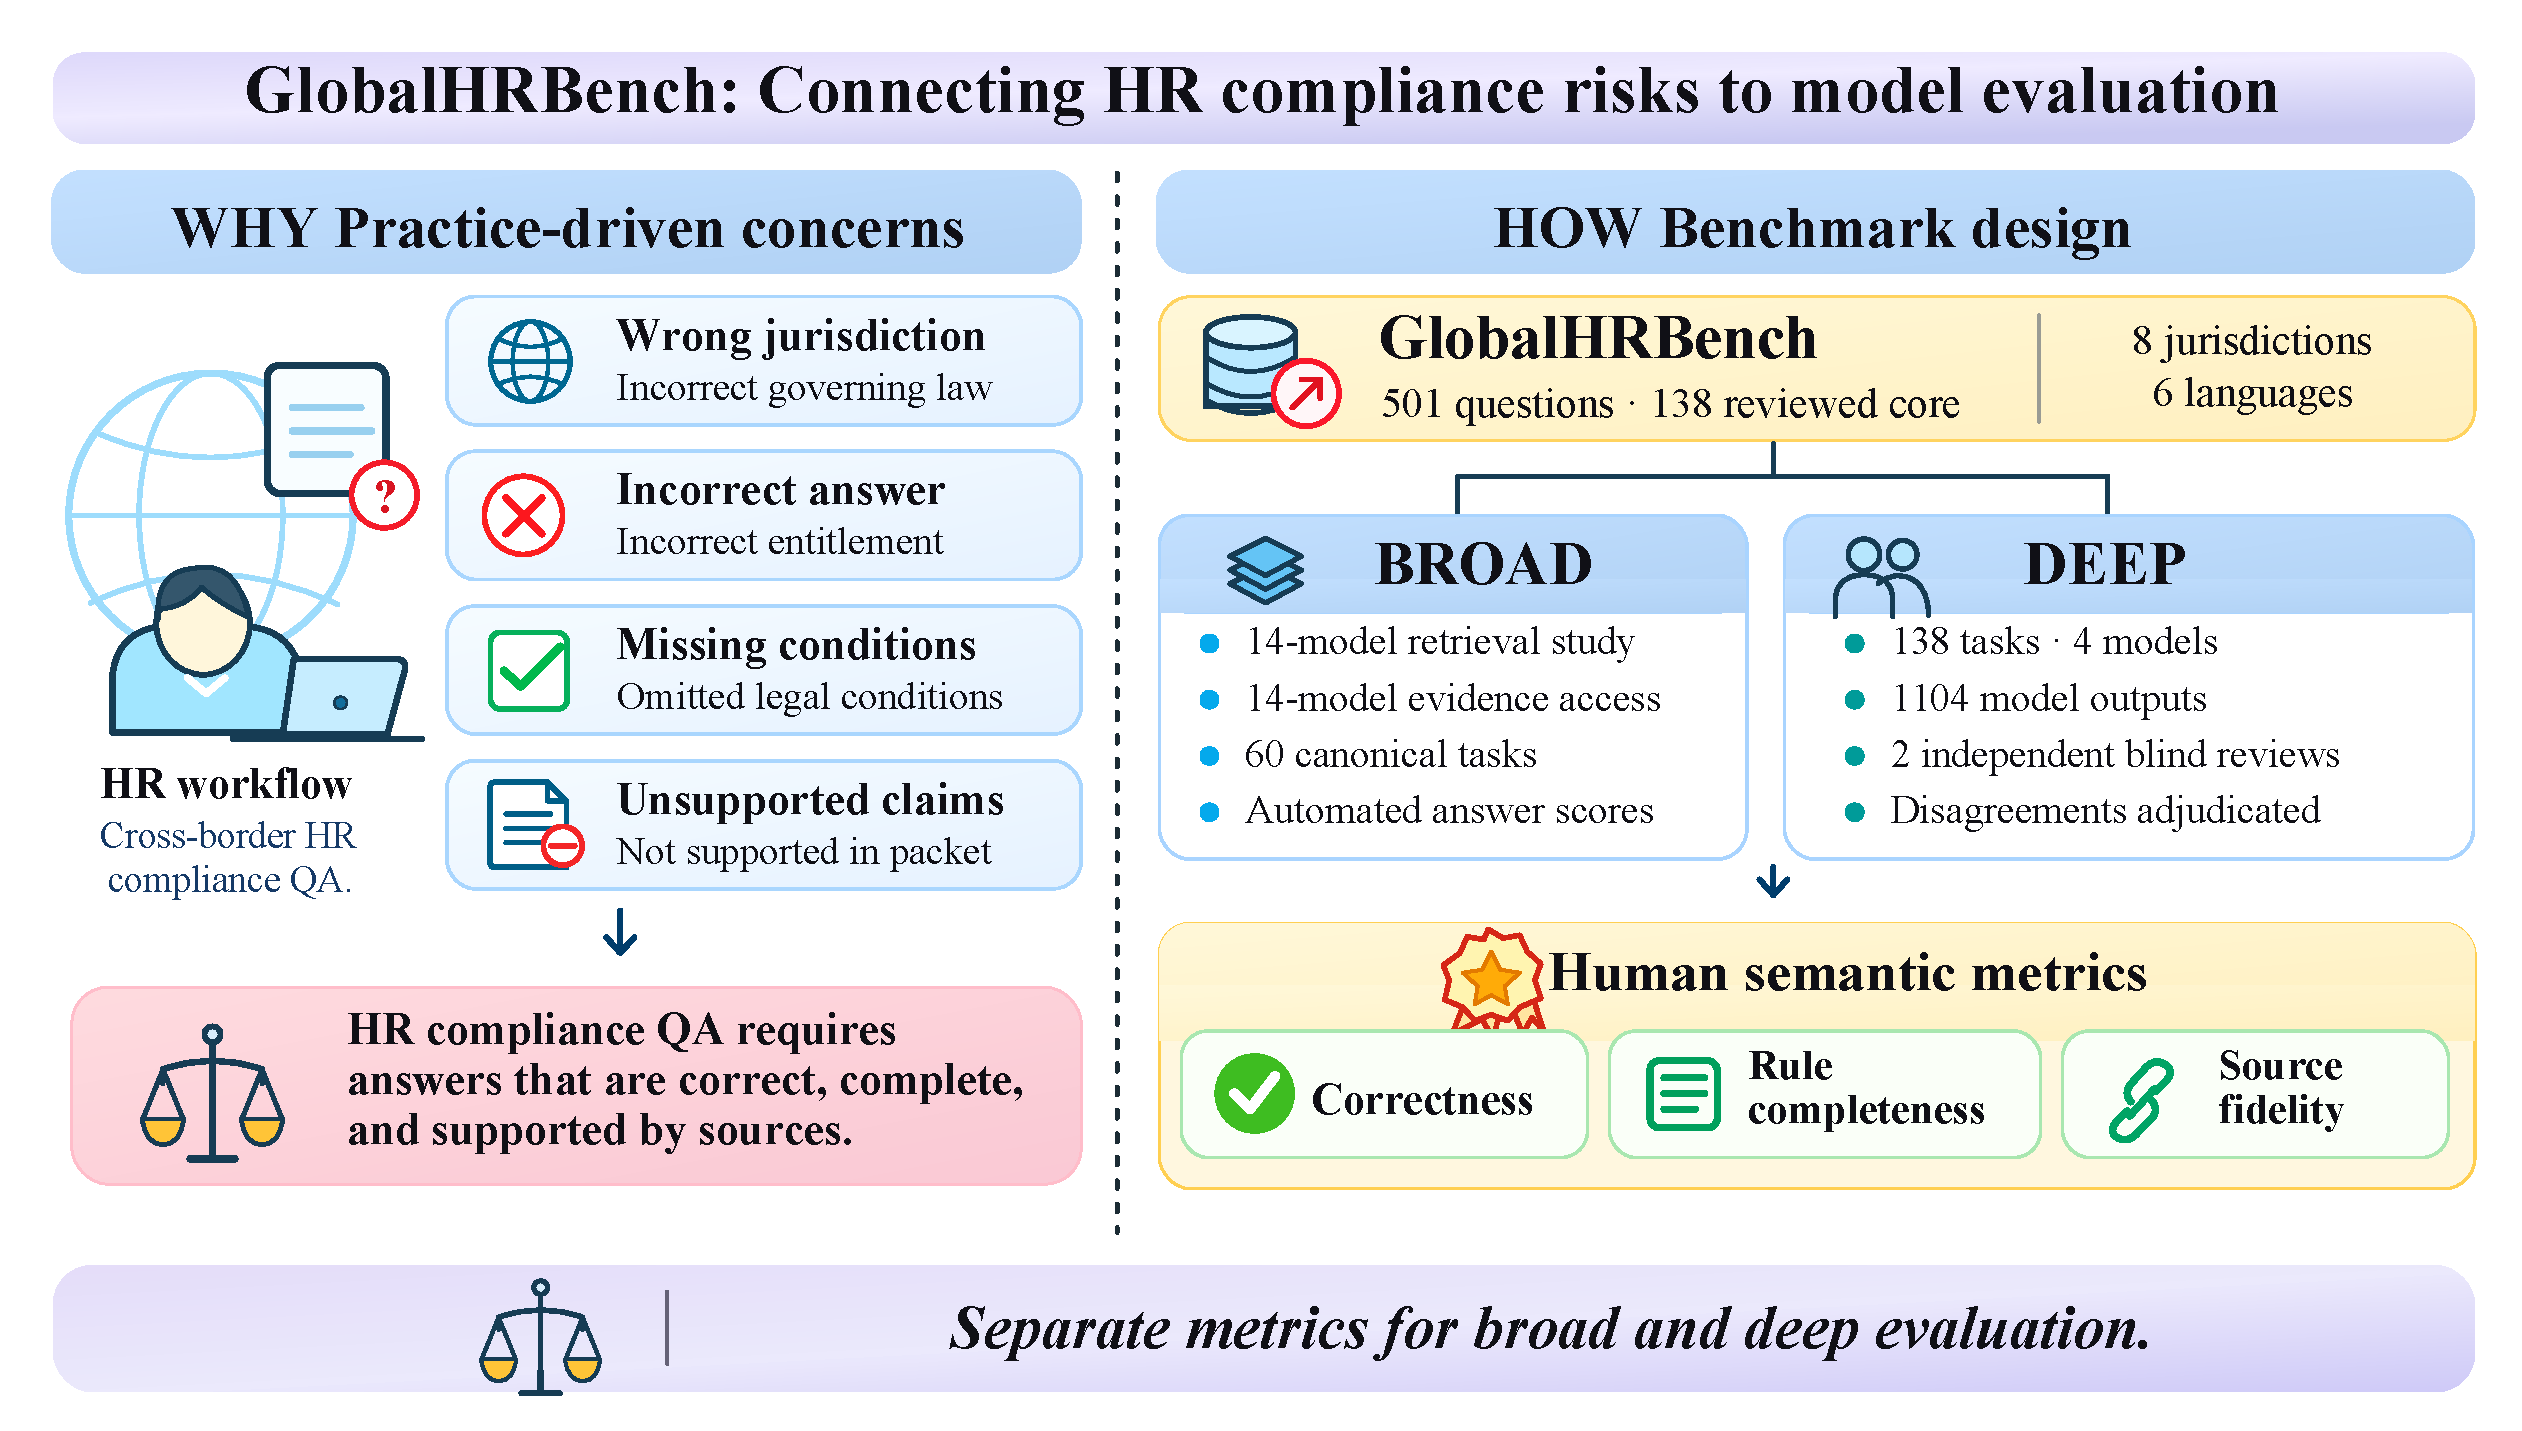
\includegraphics[width=\textwidth]{assets/GlobalHRBench_Overview_Vector.pdf}
\caption{\claim{CAPARCH}{GlobalHRBench connects HR compliance risks to broad model evaluation and deep human validation. The source-linked resource contains 501 unique questions, including a 138-question reviewed core. Automated target-answer matching supports model comparisons; human review separately assesses correctness, required-rule completeness, and source fidelity.}}
\label{fig:architecture}
\end{figure*}

\begin{figure*}[t]
\centering
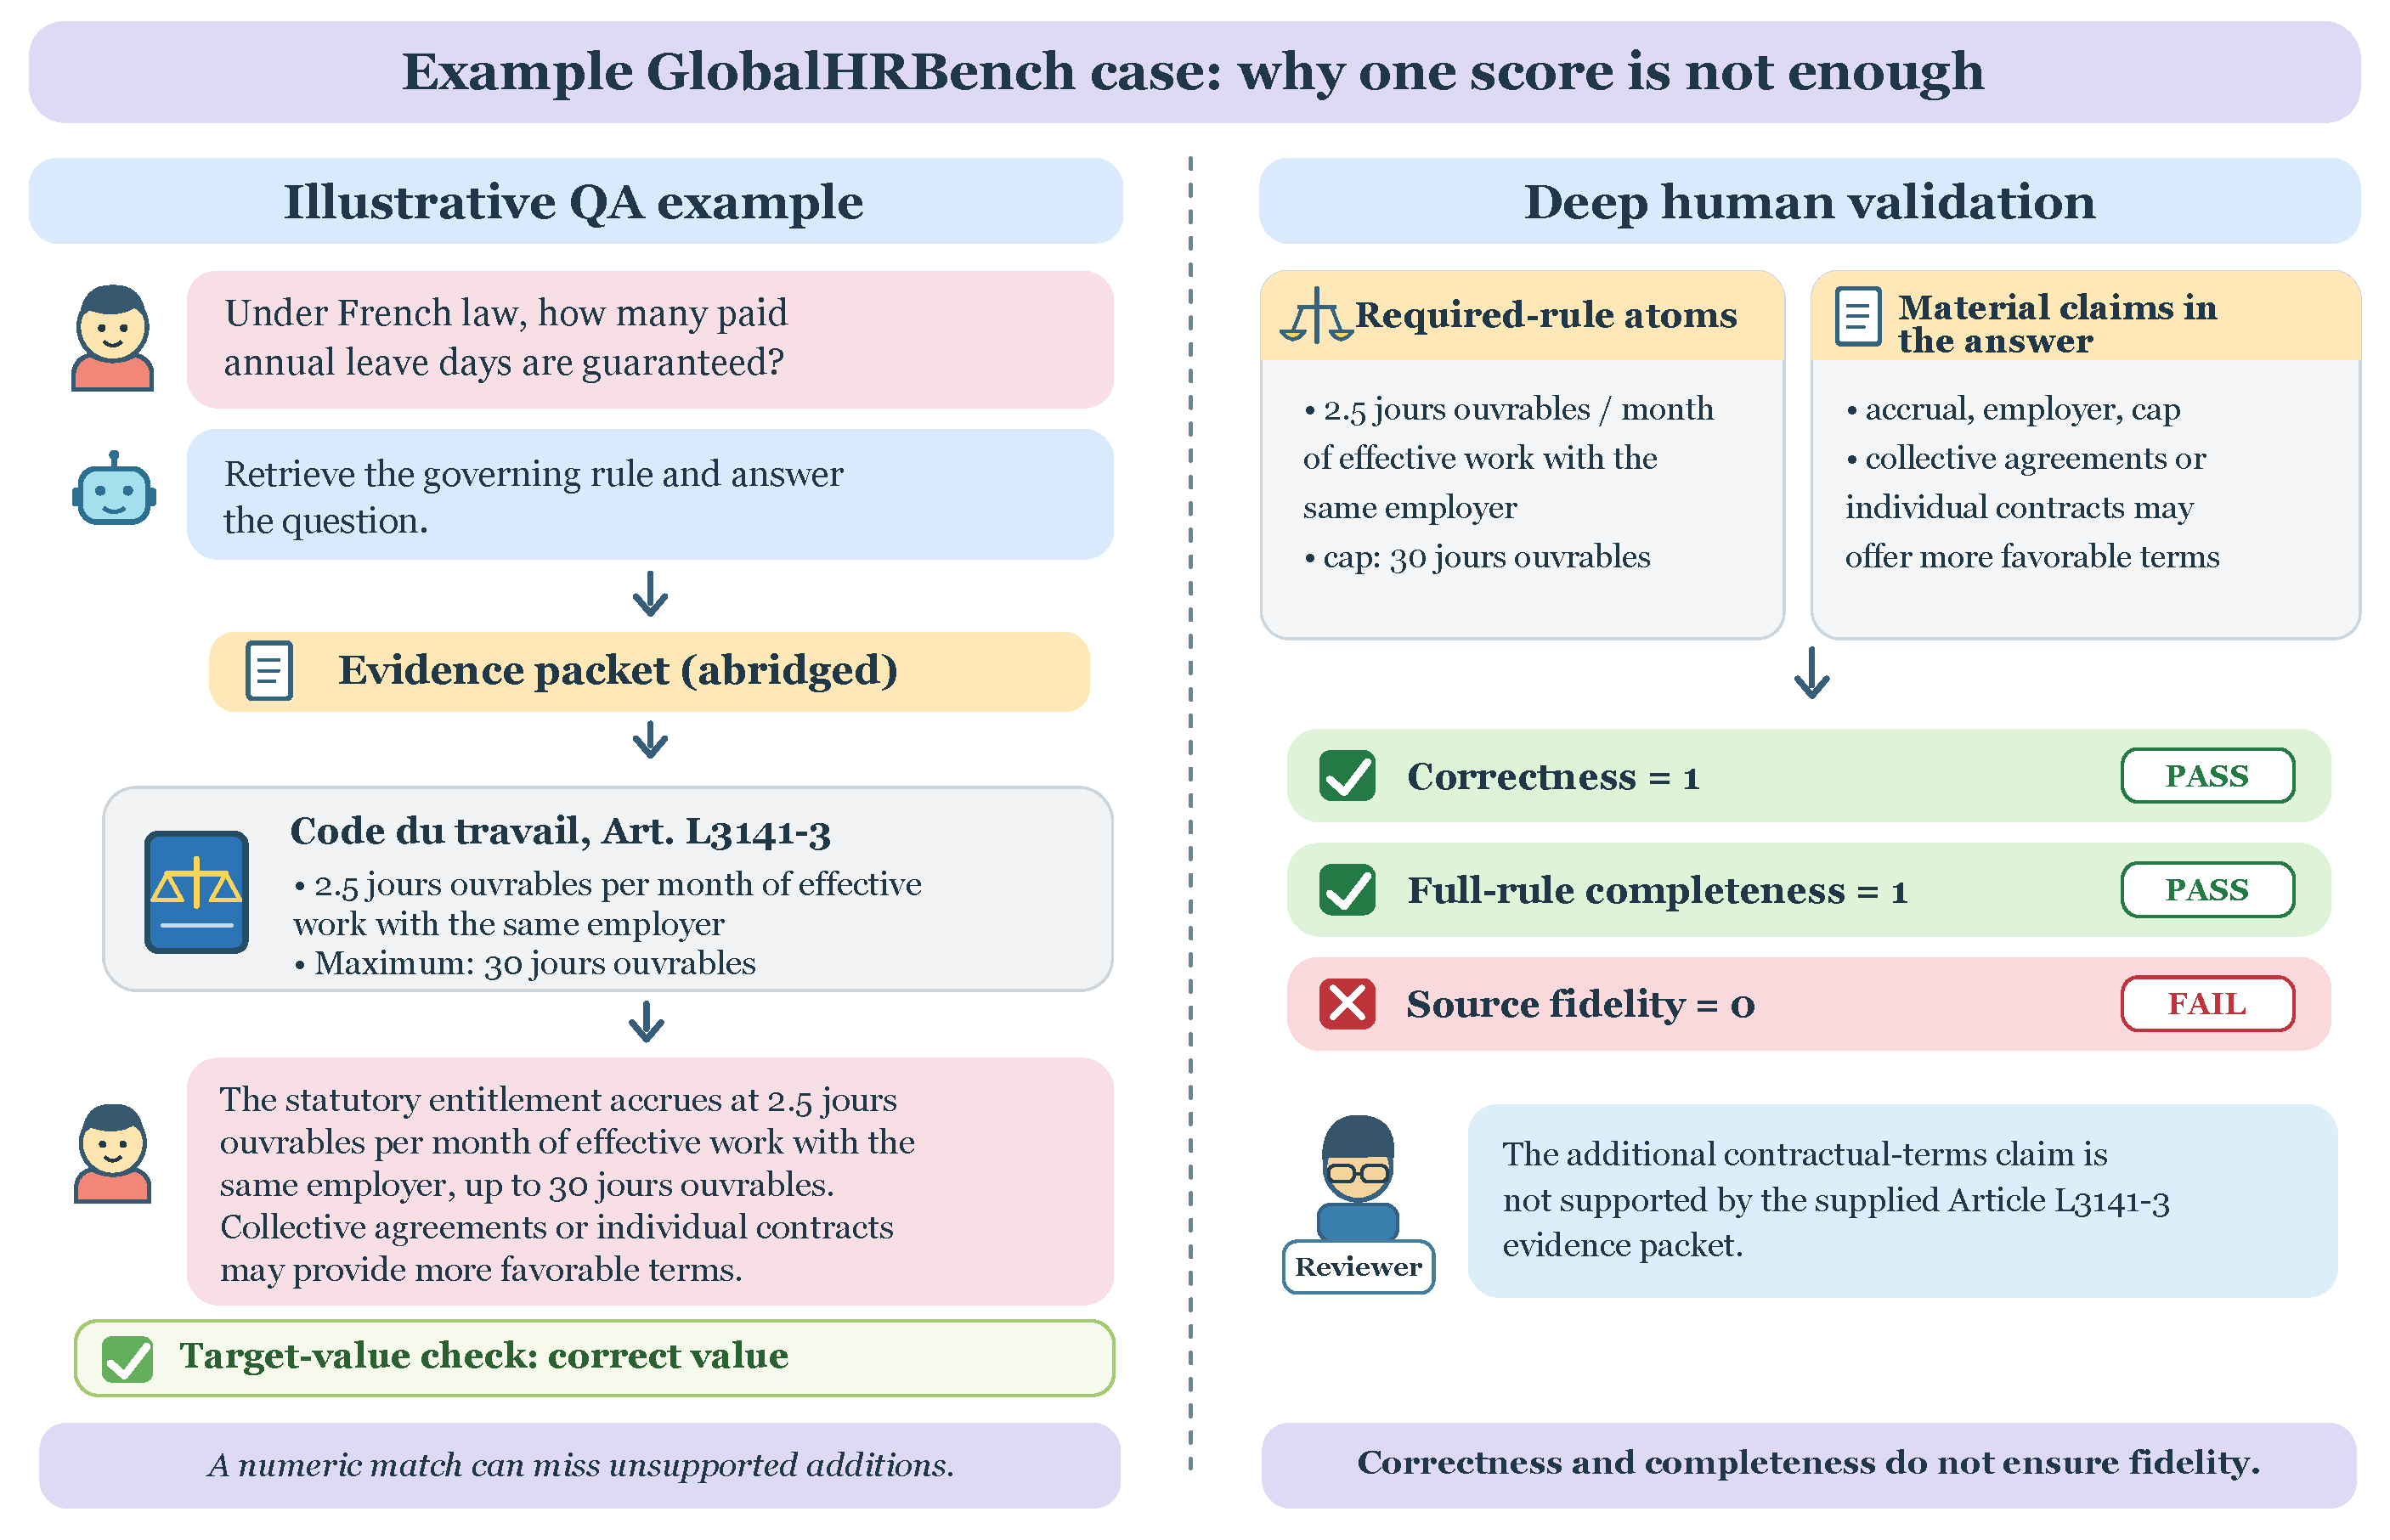
\includegraphics[width=\textwidth]{assets/GlobalHRBench_Example_Case_Vector.pdf}
\caption{\claim{CAPCASE}{Illustration of the French leave case (Section~\ref{sec:rq3}). The answer is paraphrased and the evidence abridged for readability. Human scores refer to the complete original response, including its unsupported qualification. The left panel illustrates target-value matching, not an additional scored run. Fidelity is relative to the supplied evidence.}}
\label{fig:case}
\end{figure*}

\section{Related Work}
\claim{RELATED}{\textbf{Legal and employment-law benchmarks.} LegalBench covers diverse forms of legal reasoning \citep{guha2023legalbench}. LexGLUE and LEXTREME organize legal language-understanding tasks in English and across multiple languages \citep{chalkidis2022lexglue,niklaus2023lextreme}; LawBench evaluates Chinese legal knowledge and application \citep{fei2024lawbench}. CUAD supports expert-annotated extraction of salient contract provisions \citep{hendrycks2021cuad}. LaborBench is the closest domain precedent: it derives unemployment-insurance QA from comparisons of U.S. state laws and pairs it with a statutory corpus \citep{hariri2025laborbench}. GlobalHRBench focuses on cross-jurisdiction employment-law QA, linking each reviewed question to the legal propositions an answer must preserve. Its multilingual coverage serves this task rather than a general legal-understanding leaderboard.}

\claim{RELATED}{\textbf{Legal retrieval and rule conditions.} LegalBench-RAG evaluates retrieval of precise legal text \citep{pipitone2024legalbenchrag}; Bar Exam QA and Housing Statute QA test retrieval grounded in legal reasoning \citep{zheng2025legalretrieval}. Legal RAG Bench evaluates retrieval, correctness, and groundedness in criminal-law QA using a model judge \citep{butler2026legalragbench}. ContractNLI pairs document-level entailment judgments with supporting contract spans \citep{koreeda2021contractnli}. ShARC studies rule interpretation and clarification \citep{saeidi2018interpretation}, while ConditionalQA represents conditions on answer applicability \citep{sun2022conditionalqa}. These tasks motivate evaluating the conditions that make an employment-law answer complete.}

\claim{RELATED}{\textbf{Answer support and evaluation.} RGB probes robustness to noisy or counterfactual evidence, rejection of unanswerable queries, and information integration \citep{chen2024rgb}. ALCE separates answer correctness from citation quality \citep{gao2023alce}. FActScore measures support for atomic facts in generated text \citep{min2023factscore}; RAGAs and ARES evaluate retrieval and answer quality using automated judges \citep{es2024ragas,saadfalcon2024ares}. RAGTruth provides human annotations of unsupported or contradictory content at the response and word levels \citep{niu2024ragtruth}. GlobalHRBench combines independently reviewed required-rule atoms, accepted AND/OR answer paths, and source-span judgments for all material claims. This distinguishes missing required conditions from unsupported additions within the same answer. Our contribution is the multilingual employment-law resource and its structured human evaluation, rather than the separation of answer quality and grounding alone.}

\section{Resource and Reviewed Core}
\claim{DATASET}{GlobalHRBench contains \RNResource{} unique questions across eight jurisdictions and six question languages: \RNARRUnique{} questions in the base collection and 78 reviewed multilingual extension questions. The \RNCore{}-question reviewed core combines \RNARRCore{} canonical tasks from that collection with all 78 extension questions, covering seven jurisdictions and all six languages (Figure~\ref{fig:coverage}). Each core record links the question and reference answer to a jurisdiction, language, required-rule atoms, and evidence IDs. The evidence inventory contains \RNPrimary{} primary passages, 37 from the base collection and 39 from the extension, plus five supplementary records. A passage is a provision-level evidence unit; several passages may belong to the same legal instrument. Question and source languages may differ.}

\claim{PROVENANCE}{Local legal and HR experts reviewed the question-relevant legal provisions, reference answers, and required-rule annotations against the law in effect on September 17, 2026. We retain source snapshots, effective-date evidence, and review records to support traceability. Appendix~\ref{app:arr-details} describes the question versions used in each evaluation.}

\begin{figure*}[t]
\centering
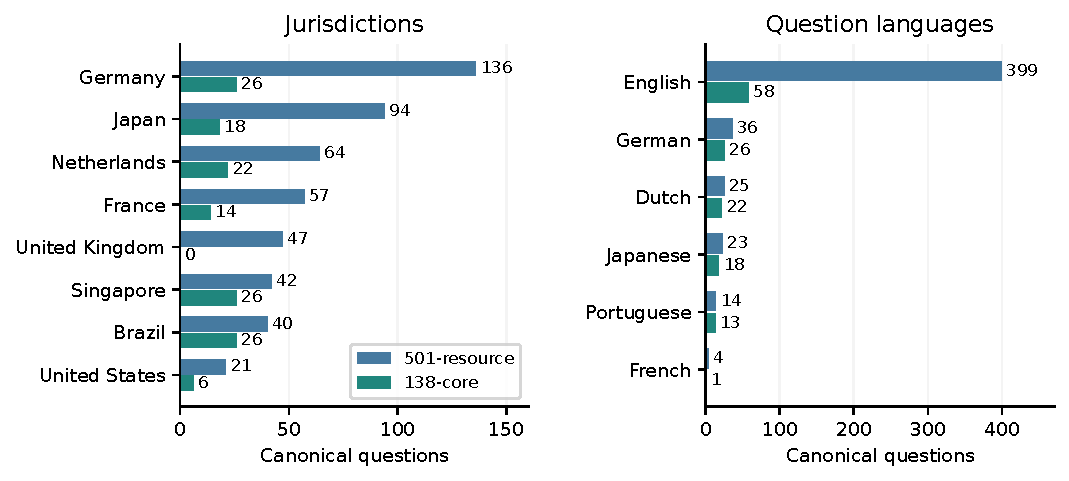
\includegraphics[width=\textwidth]{assets/figure2_coverage.pdf}
\caption{\claim{CAPCOVERAGE}{Jurisdiction and language coverage of the \RNResource{}-question resource and \RNCore{}-question reviewed core. Counts refer to canonical questions. The broad comparison includes 58 English, one French, and one Portuguese question; the reviewed core covers all six languages. Coverage is uneven, and language and jurisdiction are substantially confounded.}}
\label{fig:coverage}
\end{figure*}

\section{Evaluation Design: Breadth and Depth}
\begin{table*}[t]
\centering\small\setlength{\tabcolsep}{5pt}
\claim{DESIGN}{
\begin{tabular}{p{.21\textwidth}p{.13\textwidth}p{.24\textwidth}p{.31\textwidth}}
\toprule
Study & Tasks / models & Evidence comparison & Measurement and purpose \\
\midrule
Retrieval comparison & \RNARRCore{} / 14 & BM25 vs country routing & Target-answer score; model and retrieval differences \\
Evidence access & \RNARRCore{} / 7 & Closed / BM25 / designated & Target-answer score; performance differences across evidence conditions \\
Human validation & \RNCore{} / 4 & C: public-cue / D: designated & Correctness, rule completeness, and source fidelity \\
\bottomrule
\end{tabular}
}
\caption{\claim{CAPSTUDY}{Evaluation design. All task counts exclude exact aliases. Each broad study uses its own matched model outputs and BM25 baseline. A separate \RNARRUnique{}-question analysis describes resource-wide performance.}}
\label{tab:studies}
\end{table*}

\claim{DESIGN}{Table~\ref{tab:studies} summarizes three complementary comparisons. The fourteen-model study tests whether jurisdiction-aware retrieval improves performance across models. The seven-model study compares closed-book, retrieved, and designated evidence to examine the role of evidence access. The four-model human evaluation asks what these answer scores leave unresolved: whether responses preserve the required rule and support every material claim. Broad results use automated target-answer matching on the base question versions; human results use semantic judgments on the reviewed core. We analyze each study within its own protocol and do not pool scores across layers. A six-model structured-output diagnostic is reported separately in Appendix~\ref{app:operational}.}



\subsection{Broad model and evidence comparisons}
\claim{ROUTING}{For the broad retrieval comparison, country routing filters BM25 results to the unique country recognized in the public question, with global fallback when no unique country is found. It uses 37 primary passages and no gold jurisdiction labels. In the human evaluation, condition C uses fixed public-question and context cues to route BM25 over all \RNPrimary{} primary passages, again with global fallback for absent or ambiguous cues. Condition D supplies the designated evidence and required dependencies. Appendix~\ref{app:arr-details} distinguishes this filtering approach from an additional offline score-bonus reranker.}

\claim{ARRMETRIC}{The automated \emph{target-answer score} checks quantities, units, and polarity where available, and otherwise uses answer-text matching with lexical heuristics. It measures agreement with the reference target rather than human judgment of the full answer. Citation overlap measures matching source IDs. Each comparison keeps its original scorer and failure denominator.}

\claim{ARRPROTOCOL}{Seven models are evaluated under closed-book, BM25, and designated evidence; fourteen are evaluated under matched BM25 and country routing. Each model in the routing study has a BM25 baseline from the same batch. Appendix~\ref{app:arr-details} lists models and protocol details; the materials retain endpoint IDs, response normalization, and the failed-request replay policy.}

\begin{figure*}[t]
\centering
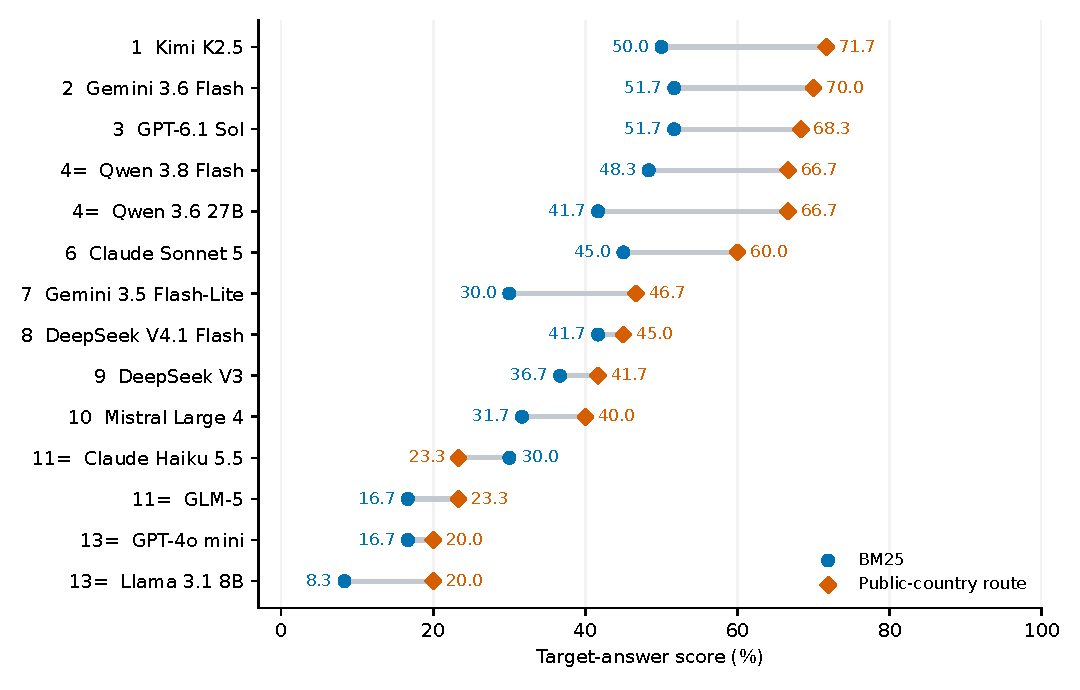
\includegraphics[width=\textwidth]{assets/retrieval_models.pdf}
\caption{\claim{CAPRANK}{Fourteen-model target-answer scores on the same \RNARRCore{} canonical tasks. Each model is evaluated with BM25 and public-country routing, with failures retained in the denominator. Models are ordered by routed score, then BM25 score; equal scores retain tied ranks. Table~\ref{tab:twelve-details} reports exact scores and alias/group sensitivities.}}
\label{fig:twelve}
\end{figure*}

\subsection{Canonical aggregation and uncertainty}
\claim{DEDUP}{We use one fixed representative per canonical task, chosen independently of model outcomes, across every model and condition. This yields \RNARRCore{} tasks per main comparison and \RNModelPairs{} paired model--task comparisons in the fourteen-model study. An alias-balanced sensitivity analysis first averages outputs within each task for the original twelve-model cohort; the two additions use the fixed canonical representatives. The \RNARRUnique{}-task resource-wide analysis includes development material and is descriptive rather than held out.}

\claim{STATISTICS}{We report question-weighted and equal-source-group means for the broad comparisons. Paired bootstrap intervals resample the five source groups, with models fixed (5,000 replicates; seed 31). The human evaluation uses question, equal-fact-group, and dependency-group analyses (2,000 paired whole-group replicates; seed 20261105). Its \RNFact{} fact groups, \RNDependency{} dependency groups, \RNSource{} primary-source groups, and \RNInstrument{} instruments describe different sources of dependence. These intervals summarize uncertainty within the constructed benchmark; model-by-question output counts are not independent sample sizes.}

\begin{figure*}[t]
\centering
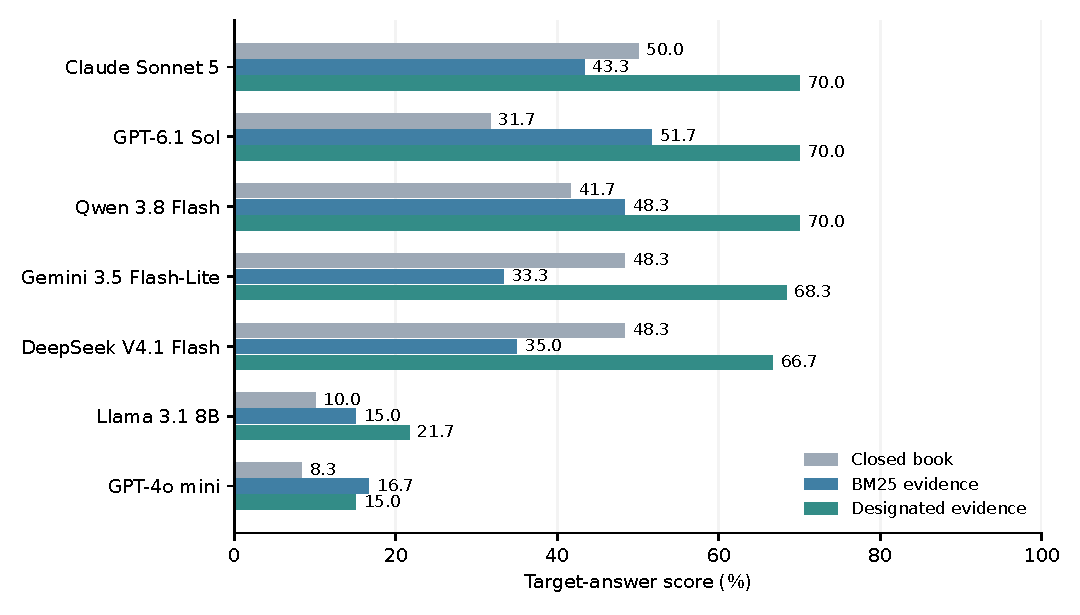
\includegraphics[width=\textwidth]{assets/evidence_models.pdf}
\caption{\claim{CAPFIVE}{Seven-model closed-book/BM25/designated-evidence comparison on \RNARRCore{} canonical tasks from the base collection per cell. Every bar aggregates row-level scores from the same target-answer scorer; the same predetermined task representative is used across all conditions. Designated evidence supplies governing material but does not guarantee an accurate interpretation.}}
\label{fig:five}
\par\medskip\begingroup\makeatletter\def\@captype{table}\makeatother
\centering\small
\begin{tabular}{lrrr}
\toprule
Model & Closed & BM25 & Designated \\
\midrule
claude-sonnet-5 & 48.0 & 23.6 & 56.7 \\
gemini-3.5-flash-lite & 45.2 & 16.3 & 58.2 \\
llama-3.1-8b-instruct & 9.5 & 11.3 & 23.2 \\
gpt-4o-mini & 11.8 & 7.3 & 20.8 \\
qwen3.8-flash & 48.0 & 26.7 & 60.3 \\
\bottomrule
\end{tabular}

\caption{\claim{CAPARRFULL}{Resource-wide five-model target-answer scores (\%) over all \RNARRUnique{} unique tasks in the base collection. This descriptive view includes development and test material and complements the matched \RNARRCore{}-task main comparison; it is not an additional held-out test. Each canonical task has equal weight and failures remain in the denominator.}}
\label{tab:arr-full}
\endgroup
\end{figure*}







\subsection{Human semantic evaluation}
\claim{HUMANPROTOCOL}{We evaluate GPT-4.1 mini, Qwen3.8 Flash, GPT-6.1 Sol, and DeepSeek V4.1 Flash under conditions C and D. The first two were selected before inspecting their outputs; we subsequently extended the same frozen questions, prompts, evidence packets, and human scoring protocol to the latter two. Each model--condition cell includes all \RNCore{} reviewed questions, yielding \RNAudit{} outputs and \RNForms{} independent review forms. GPT-4.1 mini is distinct from GPT-4o mini in the broad study. The original pair was run on 6 November 2026 UTC and the added pair on 14 November. Human-evaluation requests used a 1,024-token cap with no client retries; Appendix~\ref{app:human-settings} gives the native model settings. Appendix~\ref{app:operational} reports provider-control deviations in the original generation matrix.}

\claim{HUMANPROTOCOL}{We assigned separately randomized review packets to jurisdiction-specific legal and HR consultants from partner firms. Model and condition labels were hidden behind opaque IDs. Each output received two independent reviews; reviewers could not see one another's scores or discuss initial judgments before submitting them. Forms contained no prefilled AI scores. AI assistance was permitted for drafting review text, but every item required individual human examination and approval. Actual auxiliary-tool use was not systematically recorded. Correctness references were presented separately from the evidence used to judge source fidelity. All disagreements and unclear judgments were referred for adjudication, producing final labels for all \RNAudit{} outputs after \RNAdj{} adjudications.}

\claim{HUMANMETRICS}{\textbf{Correctness} assesses the requested full answer, including polarity, units, scope and qualifications; every core item uses human judgment. \textbf{Required-rule completeness} labels required atoms covered, contradicted, absent or unclear; covered/contradicted labels require literal quotations. Question-given premises and supplementary atoms incur no omission penalty. Full completeness requires an entirely covered accepted path in frozen AND/OR logic. Fractional coverage uses the path with maximum covered fraction, with canonical-ID tie-breaking; inapplicable roles are N/A.}

\claim{HUMANMETRICS}{\textbf{Whole-answer source fidelity} assesses all material legal claims, including additions beyond required atoms. Reviewers enumerate and quote claims; support requires exact source spans from the supplied packet. Any unsupported material claim makes the answer unsupported; otherwise unclear claims yield unclear fidelity, all supported claims yield supported fidelity, and empty inventories require explanation. Unsupported is packet-relative, not universal legal falsity. Literal checks verify quote integrity, not entailment or exhaustive enumeration.}

\claim{HUMANMETRICS}{Frozen protocol-adjusted metrics assign failures, invalid/malformed output, abstention and insufficient evidence zero on eligible success measures. Raw human judgments are preserved for joint semantic analysis. A format zero does not establish legal error; the six-model response-contract diagnostic is excluded from the semantic leaderboard.}



\section{Broad Benchmark Results}

\subsection{RQ1: Retrieval and the fourteen-model comparison}
\claim{RQONE}{On the \RNARRCore{} canonical tasks from the base collection, online public-country filtering increases primary-evidence Hit@5 from \RBMHit\% to \RRouteHit\% and reduces wrong-jurisdiction top-one results from \RBMWrong\% to \RRouteWrong\%. Appendix Table~\ref{tab:arr-retrieval} includes Hit@1, reciprocal rank, and equal-group results. These measures concern the original governing primary passages, with the original corpus. Filtering changes both evidence identity and, when fewer passages remain, packet size.}



\claim{BROADMODEL}{Across the fourteen models, the mean target-answer score rises from \RBroadBM\% with BM25 to \RBroadRoute\% with country routing (Figure~\ref{fig:twelve}). The question-weighted gain is \RBroadGain{} percentage points; the equal-source-group gain is \RBroadGroupGain{} points, with descriptive interval [\RBroadLow{}, \RBroadHigh{}]. Across \RNModelPairs{} paired comparisons, routing produces \RRoutingWins{} wins, \RRoutingTies{} ties, and \RRoutingLosses{} losses relative to BM25. \RNPositive{} models have positive question-weighted gains, while Claude Haiku 5.5 declines. Better access to governing evidence therefore helps this model set on average, with substantial variation across models.}

\claim{BROADMODEL}{Kimi K2.5 has the highest routed point estimate (71.7\%). This ordering describes performance on the specified cohort and target-answer metric. Appendix~\ref{app:arr-details} reports equal-group sensitivities for all fourteen models and alias-balanced estimates for the original twelve.}



\subsection{RQ2: Seven models under three evidence conditions}


\claim{RQTWO}{Across the seven models on the canonical core, the target-answer score is \RFiveClosed\% closed-book, \RFiveBM\% with BM25, and \RFiveGold\% with designated evidence (Figure~\ref{fig:five}). This matrix exposes substantial model and evidence-condition variation. Claude Sonnet 5, GPT-6.1 Sol and Qwen 3.8 Flash each reach 70.0\% with designated evidence. GPT-4o mini does not improve from BM25 to designated evidence in this cell. We therefore treat designated evidence as an evidence-access diagnostic rather than an assured empirical ceiling.}

\claim{RQTWO}{Retrieval success helps explain the BM25 results. On the 32 canonical retrieval hits, mean seven-model performance is \RSliceHitBM\% with BM25 versus \RSliceHitClosed\% closed-book. On the 28 misses, the corresponding scores are \RSliceMissBM\% and \RSliceMissClosed\%. These descriptive strata show how an overall RAG score can conceal different behavior when governing evidence is present or absent. They are not randomized treatment groups. Table~\ref{tab:arr-evidence-ci} reports paired source-group sensitivities.}





\claim{RQTWO}{The \RNARRUnique{}-question view (Table~\ref{tab:arr-full}) retains the original five-model cohort and includes development material. Partial applicability-slot scores for that cohort are retained in Appendix~\ref{app:sensitivities}; their limited extractor cannot quantify semantic omissions. The human layer directly evaluates completeness and fidelity.}



\begin{figure*}[t]
\centering
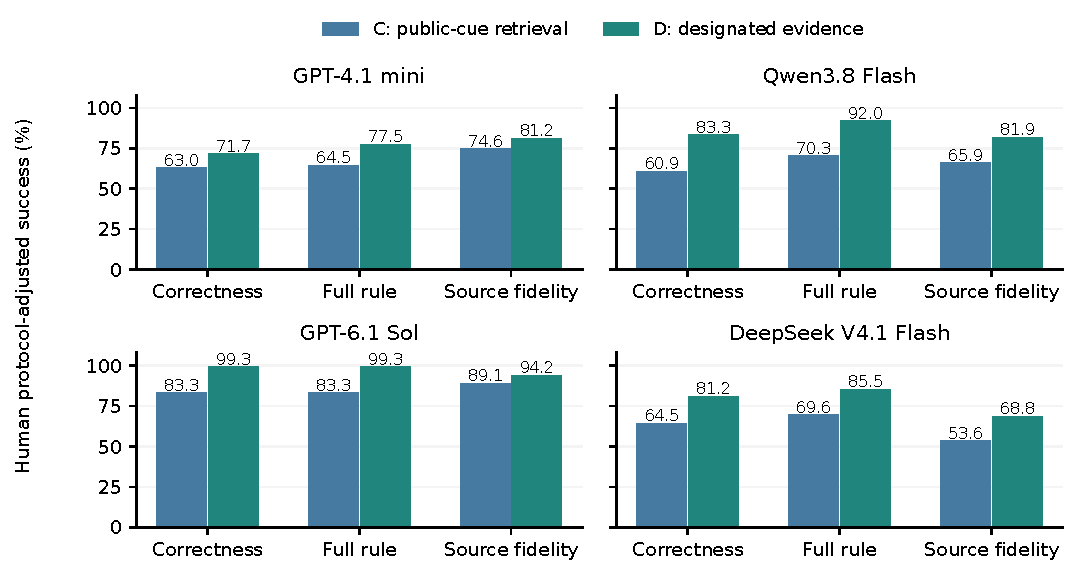
\includegraphics[width=\textwidth]{assets/human_semantics.pdf}
\caption{\claim{CAPHUMAN}{Human semantic evaluation under public-cue retrieval (C) and designated evidence (D), with \RNCore{} questions per model and condition. Bars report question-weighted, protocol-adjusted correctness, full-rule completeness, and source fidelity; failures remain in the denominator.}}
\label{fig:human}
\par\medskip\begingroup\makeatletter\def\@captype{table}\makeatother
\centering\small
\begin{tabular}{llrrrrr}
\toprule
Model & Arm & Correct & Value & Qualification & Full rule & Fidelity \\
\midrule
GPT-4.1 mini & C & 63.0 & 86.6 & 76.0 & 64.5 & 74.6 \\
GPT-4.1 mini & D & 71.7 & 96.6 & 84.2 & 77.5 & 81.2 \\
Qwen3.8 Flash & C & 60.9 & 89.7 & 75.2 & 70.3 & 65.9 \\
Qwen3.8 Flash & D & 83.3 & 98.7 & 96.8 & 92.0 & 81.9 \\
GPT-6.1 Sol & C & 83.3 & 93.5 & 78.6 & 83.3 & 89.1 \\
GPT-6.1 Sol & D & 99.3 & 99.2 & 98.8 & 99.3 & 94.2 \\
DeepSeek V4.1 Flash & C & 64.5 & 80.5 & 70.1 & 69.6 & 53.6 \\
DeepSeek V4.1 Flash & D & 81.2 & 93.7 & 78.5 & 85.5 & 68.8 \\
\bottomrule
\end{tabular}

\caption{\claim{CAPHUMANVALUES}{Human outcomes (\%). Correctness, full-rule completeness, and fidelity use \RNCore{} questions per cell. Value and qualification coverage use 126 and 85 eligible questions, respectively. Structurally inapplicable roles are excluded; failures on eligible questions remain zero.}}
\label{tab:human-values}
\endgroup
\end{figure*}

\section{Deep Human Semantic Validation}
\subsection{RQ2: Evidence access under full-answer review}
\claim{DEEPRESULT}{Figure~\ref{fig:human} evaluates semantic outcomes over all \RNCore{} reviewed questions. Correctness rises from \ROCCorrect\% under C to \RODCorrect\% under D for GPT-4.1 mini, from \RQCCorrect\% to \RQDCorrect\% for Qwen3.8 Flash, from \RSCCorrect\% to \RSDCorrect\% for GPT-6.1 Sol, and from \RDCCorrect\% to \RDDCorrect\% for DeepSeek V4.1 Flash. These matched C/D comparisons complement the broad evidence-access comparison with full-answer human judgments.}

\claim{DEEPRESULT}{For GPT-6.1 Sol, correctness under retrieval is \RSCCorrect\% across all \RNCore{} questions but reaches \RSCAvailableCorrect\% among the \RSCAvailableN{} questions for which the retrieved packet contains all required evidence. This suggests that missing governing evidence is an important source of error, although the evidence-available subset is descriptive rather than a randomized comparison.}


\claim{DEEPRESULT}{Grouping changes the interpretation of improvement. GPT-4.1 mini's equal-fact-group correctness is \ROCGroupCorrect\% under C and \RODGroupCorrect\% under D, even though its question-weighted estimate increases. Qwen improves from \RQCGroupCorrect\% to \RQDGroupCorrect\% under equal-fact-group weighting. Both added models also improve under equal-fact-group weighting: GPT-6.1 Sol rises from \RSCGroupCorrect\% to \RSDGroupCorrect\%, and DeepSeek from \RDCGroupCorrect\% to \RDDGroupCorrect\%. The appendix retains paired group sensitivities, value/qualification denominators, and evidence-available subsets. The core's language slices are also reported, exposing uneven performance without treating language as an isolated causal factor.}

\claim{DEEPRESULT}{Under designated evidence, GPT-4.1 mini reaches \RODValue\% value coverage and \RODQual\% qualification coverage, but \RODFull\% full-rule completeness and \RODFidelity\% source fidelity. Qwen reaches \RQDValue\%, \RQDQual\%, \RQDFull\%, and \RQDFidelity\%, respectively (Table~\ref{tab:human-values}). GPT-6.1 Sol reaches \RSDFull\% full-rule completeness but \RSDFidelity\% fidelity; DeepSeek reaches \RDDFull\% and \RDDFidelity\%. Full-rule coverage does not ensure correctness: an adjudicated Qwen answer covered the required Dutch employment information deadlines but overstated a separate notification duty by omitting its exceptions.}



\begin{figure*}[t]
\centering
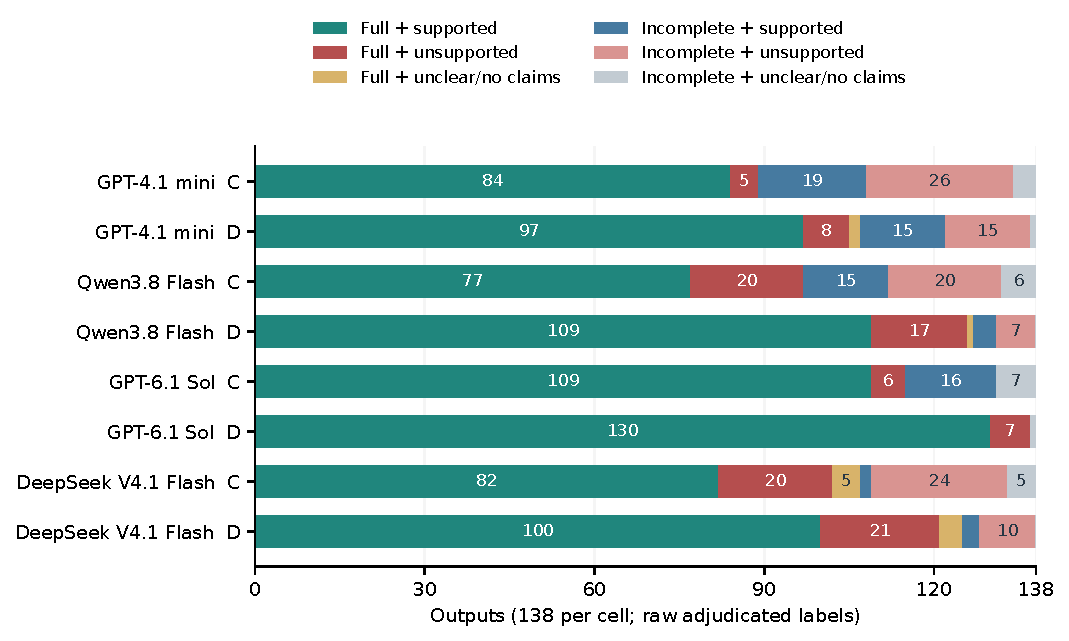
\includegraphics[width=\textwidth]{assets/joint_failures.pdf}
\caption{\claim{CAPFAIL}{Joint rule-completeness and source-fidelity judgments, using raw adjudicated labels. Full/incomplete concerns required-rule coverage; supported/unsupported concerns all material claims. Red segments identify complete answers with unsupported additions. This descriptive cross-tab complements the protocol-adjusted rates in Figure~\ref{fig:human}.}}
\label{fig:joint}
\end{figure*}

\subsection{RQ3: Failures an ordinary answer score misses}
\label{sec:rq3}

\claim{JOINTFAIL}{Figure~\ref{fig:joint} shows the distinction within individual answers. Under designated evidence, \RODUnsupported{} GPT-4.1 mini and \RQDUnsupported{} Qwen answers cover the complete required rule yet include an unsupported material claim. The same pattern appears in \RSDUnsupported{} GPT-6.1 Sol and \RDDUnsupported{} DeepSeek answers. Under retrieval, these counts are \ROCUnsupported{}, \RQCUnsupported{}, \RSCUnsupported{}, and \RDCUnsupported{}, respectively. Other answers stay faithful to their sources while omitting required rule components. Thus, a response can succeed on one dimension and fail on another.}

\begin{samepage}
\claim{CASE}{Figure~\ref{fig:case} illustrates a French annual-leave question that asks how many statutory paid leave days the law guarantees. One accepted path under Code du travail, Article L3141-3, combines accrual of 2.5 \emph{jours ouvrables} per month of effective work with the same employer and a total cap of 30. Qwen3.8 Flash covered both atoms under designated evidence, but added that ``collective agreements or individual contracts may provide more favorable terms.'' The supplied article did not support that addition. Adjudicated scores: correctness 1, full-rule completeness 1, and source fidelity 0. Fidelity here is packet-relative, not a judgment of legal falsity.}
\par\end{samepage}

\subsection{Reviewer agreement}
\claim{RELIABILITY}{Before adjudication, exact agreement is \RAgreeCorrect\% for correctness, \RAgreeFidelity\% for whole-answer fidelity, and \RAgreeAtom\% for required-atom labels; the corresponding descriptive Cohen's kappas are \RKappaCorrect{}, \RKappaFidelity{}, and \RKappaAtom{} (Table~\ref{tab:agreement}). Correctness and fidelity use outputs, whereas atom agreement uses individual required-atom labels. We do not treat independently segmented claim inventories as matched units. Adjudication produces released labels but is not counted as independent agreement evidence. Marginals and directional confusion are retained.}

\begin{table}[!ht]
\centering\small
\begin{tabular}{lrrr}
\toprule
Judgment & Units & Exact (\%) & $\kappa$ \\
\midrule
Correctness & 1104 & 95.6 & 0.882 \\
Whole-answer fidelity & 1104 & 96.0 & 0.884 \\
Required-atom labels & 4176 & 98.9 & 0.933 \\
All labels per output & 1104 & 91.9 & \textemdash{} \\
\bottomrule
\end{tabular}

\caption{\claim{CAPAGREE}{Agreement before adjudication. Correctness and fidelity use outputs as units; atom agreement uses required-atom labels. The pooled review slots span jurisdiction-specific teams.}}
\label{tab:agreement}
\end{table}

\section{Discussion}
\claim{DISCUSSION}{The human evaluation shows why correctness, rule completeness, and source fidelity should be considered together. Correctness asks whether an answer resolves the requested legal issue, while rule completeness checks whether it preserves all required propositions and dependencies. Source fidelity asks whether the supplied evidence supports every material claim, including additions beyond the requested rule. These dimensions overlap, but a high score on one does not ensure success on the others. The French leave case illustrates this distinction: the answer preserves the entitlement and its required conditions, yet adds a qualification that the evidence packet does not support. A single correctness score would obscure that addition, just as fidelity alone would not reveal an omitted eligibility condition. Here, unsupported means unsupported by the supplied packet; it does not establish that a claim is legally false.}

\claim{DISCUSSION}{Evidence access and answer construction therefore require separate scrutiny. The broad retrieval results and the human evidence-access comparison suggest that obtaining governing evidence is an important part of the problem. Sol's stronger performance on questions with complete retrieved evidence further motivates examining where evidence is lost before generation. That subset is descriptive, however, and may differ in difficulty and legal content from the remaining questions. Even when the designated packet contains the required evidence, models can omit conditions or introduce unsupported qualifications. The results thus identify failures at both stages without isolating a causal contribution for each stage.}

\claim{DISCUSSION}{For RAG design, these findings motivate three checks: whether the evidence packet contains the governing provisions and dependencies, whether the answer covers the required rule, and whether each additional assertion has support. The latter two checks address what an answer omits and what it adds. They could inform systems that request missing evidence, flag incomplete conditions, or ask for revision of an unsupported qualification. Such mechanisms should preserve the distinction between a missing source and a claim contradicted by a source. These are design implications of the observed failures, not improvements evaluated in this study. Their value would need to be tested against both answer quality and the risk of suppressing useful, supported content.}

\claim{DISCUSSION}{A concrete next step is evidence-grounded fine-tuning: training models to preserve required conditions, avoid additions without support, and state the limits of an answer when evidence is insufficient. This targets behavior under a supplied evidence packet rather than general legal knowledge. A controlled evaluation would compare the same model before and after fine-tuning under matched retrieval and evidence conditions, with the same prompts and generation budgets. Training and test sets should be separated by legal source and fact group to reduce leakage through shared provisions or closely related questions. Held-out jurisdictions could then test transfer across legal systems. Evaluation should retain all three metrics and examine whether gains in fidelity come at the expense of completeness or correctness. Whether such training improves these outcomes is an open hypothesis; it cannot be assumed to compensate for missing governing evidence or replace retrieval.}

\section{Conclusion}
\claim{CONCLUSION}{GlobalHRBench combines a \RNResource{}-question multilingual employment-law resource with broad model comparisons and deep human validation on a \RNCore{}-question reviewed core. Jurisdiction-aware retrieval improves target-answer performance on average, but access to governing evidence does not ensure a complete and fully supported response. The human judgments identify failures that correctness alone misses, including rule-complete answers with unsupported additions. By linking questions, required rules, and claim-level support, GlobalHRBench provides a basis for evaluating and improving HR compliance QA beyond answer matching.}

\label{sec:content-end}
\section*{Limitations}
\claim{LIMITATIONS}{Coverage is multilingual but uneven. The broad main cohort is predominantly English, and its five source groups limit uncertainty estimation. The resource-wide analysis includes development material and is not a held-out performance estimate. Language, jurisdiction, instrument, and answer type are confounded; the reviewed core has only one French question. The resource is not a certification of current law. Group-based resampling accounts for specified dependencies without establishing statistical independence.}

\claim{LIMITATIONS}{The automated target-answer scorer uses lexical heuristics and can accept an answer with incomplete legal meaning; its applicability extractor can also miss equivalent wording. Human semantic evaluation covers four models under C/D conditions. Its findings do not establish semantic error rates for the broader model set. Reviewers may make mistakes, model or condition cues can remain in blinded content, and permitted tool assistance was not quantified. Shared review-slot codes support pooled agreement rather than person-level reliability estimates. The evaluation layers also use different question versions and generation protocols. Country filtering changes packet composition and sometimes size, so it does not isolate every retrieval mechanism. Finally, benchmark performance does not measure real HR decisions or downstream harms.}

\claim{LIMITATIONS}{The six-model structured-output diagnostic has substantial JSON failures and provider-control deviations (Appendix~\ref{app:operational}). These characterize adherence to the specified output contract rather than legal competence.}

\section*{Ethical Considerations}
\claim{ETHICS}{We developed GlobalHRBench for research on employment-law QA, not for individual legal advice or automated employment decisions. We engaged local legal and HR consultants at USD 300--500 per hour. Participants consented to research use and public release of anonymized data within the collaboration's business and research scope. We keep participant identities and contractual records confidential. We did not submit the study for institutional ethics review, and no institution issued an approval or exemption determination. We use public legal sources rather than private employee records. Source texts remain subject to their respective reuse terms; the software license does not override them. AI tools assisted drafting, translation, code, figures, and editing. Reviewers remained responsible for examining and approving each judgment.}

\bibliography{references}
\clearpage
\appendix
\section{Broad Evaluation: Protocols and Sensitivities}
\label{app:arr-details}

\claim{BASELABEL}{The internal label \texttt{ARR} in the released data and experiment files refers to the original base collection and its associated evaluation runs. We retain it in filenames and record IDs for traceability.}

\claim{ARRPROTOCOL}{The seven-model matrix uses GPT-4o mini, Gemini 3.5 Flash-Lite, Qwen3.8 Flash, Llama 3.1 8B, Claude Sonnet 5, GPT-6.1 Sol, and DeepSeek V4.1 Flash under closed-book, global BM25 top-five, and designated evidence. The fourteen-model comparison additionally includes Gemini 3.6 Flash, Claude Haiku 5.5, Qwen3.6 27B, DeepSeek V3, Mistral Large 4, Kimi K2.5, and GLM-5. Each model has matched BM25 and country-filtered responses generated in the same batch. The evidence-access matrix uses its own BM25 responses. We evaluated GPT-6.1 Sol and DeepSeek V4.1 Flash on the same fixed canonical representatives, with the existing prompts, evidence packets, response contracts, and study-specific scorers. The 423-task resource-wide analysis retains its original five models.}


\claim{NATIVECONFIG}{The two added models were evaluated on 14 November 2026 UTC. GPT-6.1 Sol uses its native reasoning interface with \texttt{reasoning\_effort=low}; \texttt{temperature} and \texttt{top\_p} are omitted. DeepSeek V4.1 Flash uses \texttt{enable\_thinking=false}, temperature zero, and top-$p$ one. Broad requests use the original 1,800-token cap, with one retry at 4,000 tokens for truncation or one retry for a transient API failure. Model IDs, exact request payloads, raw responses, and all attempts are retained.}

\claim{RQONE}{The preserved offline hybrid comparison also benefits from explicit public country cues: on the canonical core, Recall@1 changes from 43.3\% to 53.3\% and Recall@5 from 61.7\% to 91.7\%. This score-bonus reranker and the online hard-filtered BM25 are separate mechanisms. Their results support the utility of visible jurisdiction information within this resource; they do not evaluate inference of an unstated jurisdiction or justify combining all routed systems under one score.}

\claim{CANONICAL}{The base inventory contains 472 rows before deduplication. Exact task comparison identifies \RNAliases{} excess aliases across nine duplicate groups, giving \RNARRUnique{} unique tasks. The historical 82-row main comparison similarly maps to \RNARRCore{} canonical tasks, with \RNCoreAliases{} excess aliases. The crosswalk preserves every old identifier and row; no historical response is deleted. Distinct prompts, scenarios, and legally meaningful variants remain distinct questions. We count each canonical task once and additionally examine sensitivity to variation among its historical alias outputs.}

\claim{BRIDGE}{Canonical identifiers preserve task lineage across the base and reviewed versions. During core review, 21 of the 60 base question texts were revised and all 60 reference-answer fields were updated. The 78 extension questions retain their reviewed question and answer fields. Broad results use the base versions; human evaluation uses the reviewed versions. The crosswalk makes these relationships explicit without treating the two evaluations as a before/after performance comparison.}
\label{app:sensitivities}
\claim{APPSENS}{Primary estimates use the fixed canonical representative. Alias-balanced estimates average outputs within each canonical task before averaging tasks; equal-group estimates average source-group means. Equal-group results cover all fourteen models; alias-balanced results use the original twelve-model outputs. The two additions were evaluated once per fixed canonical representative, so their alias-balanced entries are unavailable. The materials also preserve pre-canonical aggregates and the ID crosswalk for tracing the deduplication.}
\begin{table*}[!t]
\centering\small
\begin{tabular}{lrrrrrl}
\toprule
Model & BM25 & Route & $\Delta_Q$ & Alias route & Group route & W/T/L \\
\midrule
Kimi K2.5 & 50.0 & 71.7 & 21.7 & 71.7 & 71.8 & 13/47/0 \\
Gemini 3.6 Flash & 51.7 & 70.0 & 18.3 & 70.0 & 70.3 & 13/45/2 \\
GPT-6.1 Sol & 51.7 & 68.3 & 16.7 & -- & 68.7 & 13/44/3 \\
Qwen 3.8 Flash & 48.3 & 66.7 & 18.3 & 66.7 & 67.5 & 11/49/0 \\
Qwen 3.6 27B & 41.7 & 66.7 & 25.0 & 66.7 & 67.4 & 16/43/1 \\
Claude Sonnet 5 & 45.0 & 60.0 & 15.0 & 60.0 & 61.0 & 13/43/4 \\
Gemini 3.5 Flash-Lite & 30.0 & 46.7 & 16.7 & 46.7 & 49.2 & 16/38/6 \\
DeepSeek V4.1 Flash & 41.7 & 45.0 & 3.3 & -- & 47.4 & 12/38/10 \\
DeepSeek V3 & 36.7 & 41.7 & 5.0 & 41.7 & 45.0 & 11/41/8 \\
Mistral Large 4 & 31.7 & 40.0 & 8.3 & 41.9 & 38.4 & 8/49/3 \\
Claude Haiku 5.5 & 30.0 & 23.3 & -6.7 & 23.3 & 26.7 & 8/40/12 \\
GLM-5 & 16.7 & 23.3 & 6.7 & 23.3 & 26.2 & 10/44/6 \\
GPT-4o mini & 16.7 & 20.0 & 3.3 & 20.0 & 25.6 & 3/56/1 \\
Llama 3.1 8B & 8.3 & 20.0 & 11.7 & 20.4 & 23.5 & 9/49/2 \\
\bottomrule
\end{tabular}

\caption{\claim{CAPALIAS}{Fourteen-model canonical comparison (\%). Each model has \RNARRCore{} paired tasks. Alias route first averages aliases within a canonical task (original twelve models; dashes indicate unavailable values); group route weights the five historical source groups equally. W/T/L counts wins, ties, and losses under the representative policy. Exact endpoint IDs and group intervals are retained in the machine-readable result summary.}}
\label{tab:twelve-details}
\end{table*}
\begin{table*}[!t]
\centering\small
\begin{tabular}{llrr}
\toprule
Retrieval & Metric & Question & Equal groups \\
\midrule
bm25 & hit at 1 & 40.0 & 36.6 \\
bm25 & hit at 5 & 53.3 & 54.3 \\
bm25 & mrr at 5 & 45.0 & 42.9 \\
bm25 & wrong jurisdiction top1 & 60.0 & 63.4 \\
country filtered & hit at 1 & 78.3 & 77.5 \\
country filtered & hit at 5 & 98.3 & 98.6 \\
country filtered & mrr at 5 & 85.1 & 84.5 \\
country filtered & wrong jurisdiction top1 & 6.7 & 9.6 \\
\bottomrule
\end{tabular}

\caption{\claim{CAPRETRIEVE}{Governing-primary retrieval on \RNARRCore{} canonical tasks. All displayed quantities are multiplied by 100, including MRR@5. These use the saved ranked passage lists; the historical model prompts preserve their original passage order, so top-ranked position should not be assumed to be prompt position.}}
\label{tab:arr-retrieval}
\end{table*}
\begin{table*}[!t]
\centering\small
\begin{tabular}{lrrl}
\toprule
Comparison & $\Delta_Q$ & $\Delta_G$ & 95\% group interval \\
\midrule
BM25 $-$ Closed & 0.7 & -0.2 & [-15.6, 15.2] \\
Designated $-$ BM25 & 19.8 & 18.2 & [4.2, 42.3] \\
Designated $-$ Closed & 20.5 & 18.0 & [3.9, 32.2] \\
\bottomrule
\end{tabular}

\caption{\claim{CAPARREVIDENCE}{Seven-model paired evidence differences, in percentage points, on the canonical core. Each bootstrap resamples the five historical source groups with models fixed. These descriptive intervals do not establish model-population effects. ``Oracle'' names the saved designated-evidence condition.}}
\label{tab:arr-evidence-ci}
\end{table*}
\begin{table*}[!t]
\centering\small
\begin{tabular}{lrrr}
\toprule
Model & Target-answer score & Partial slot F1 & Valid response \\
\midrule
claude-sonnet-5 & 70.0 & 37.0 & 93.3 \\
gemini-3.5-flash-lite & 68.3 & 0.0 & 93.3 \\
llama-3.1-8b-instruct & 21.7 & 9.0 & 98.3 \\
gpt-4o-mini & 15.0 & 0.0 & 100.0 \\
qwen3.8-flash & 70.0 & 53.8 & 93.3 \\
\bottomrule
\end{tabular}

\caption{\claim{CAPAUTOSLOTS}{Original five-model designated-evidence target-answer and partial applicability-slot scores (\%) on the canonical cohort from the base collection. Slot F1 is produced by a limited automatic extractor; the numerical difference from target-answer score is not an omission rate or a substitute for the human rule-completeness metric.}}
\end{table*}

\section{Human-Audit Subsets and Grouping}
\label{app:human-settings}
\claim{HUMANPROTOCOL}{For human-evaluation generation, GPT-4.1 mini and Qwen3.8 Flash used temperature zero and top-$p$ one. GPT-6.1 Sol uses its native reasoning interface with \texttt{reasoning\_effort=low}; temperature and top-$p$ are omitted. DeepSeek V4.1 Flash uses \texttt{enable\_thinking=false}, temperature zero, and top-$p$ one. All four models received the same task-specific messages and evidence under C and D, with a requested 1,024-token output budget and no client retries. We retain exact request payloads and all returned outputs.}
\claim{APPSENS}{The human analyses retain question and equal-fact-group weighting and the prespecified dependency sensitivity. C supplies every required evidence item for 104 questions, whereas D does so for all 138; those conditional subsets differ and their column differences are not paired treatment effects. The unclear-label sensitivity uses the original denominator and reports missing-outcome bounds instead of dropping uncertain cases. Original raw judgments remain available even when the frozen response protocol assigns a zero. For example, Qwen C has 92 raw supported judgments and 91 protocol-adjusted fidelity successes.}
\begin{table*}[tp]
\centering\small
\begin{tabular}{lrrrr}
\toprule
Metric & C: Questions & C: Equal groups & D: Questions & D: Equal groups \\
\midrule
\multicolumn{5}{l}{\textbf{GPT-4.1 mini}} \\
Correctness & 63.0 (138) & 67.0 (138) & 71.7 (138) & 67.0 (138) \\
Value coverage & 86.6 (126) & 89.8 (126) & 96.6 (126) & 97.4 (126) \\
Qualification coverage & 76.0 (85) & 86.2 (85) & 84.2 (85) & 88.8 (85) \\
Atom coverage & 81.8 (138) & 87.7 (138) & 91.8 (138) & 92.6 (138) \\
Full rule & 64.5 (138) & 67.3 (138) & 77.5 (138) & 74.0 (138) \\
Source fidelity & 74.6 (138) & 75.4 (138) & 81.2 (138) & 75.8 (138) \\
\multicolumn{5}{l}{\textbf{Qwen3.8 Flash}} \\
Correctness & 60.9 (138) & 62.7 (138) & 83.3 (138) & 77.3 (138) \\
Value coverage & 89.7 (126) & 91.5 (126) & 98.7 (126) & 98.1 (126) \\
Qualification coverage & 75.2 (85) & 85.2 (85) & 96.8 (85) & 96.0 (85) \\
Atom coverage & 84.0 (138) & 88.2 (138) & 98.0 (138) & 96.9 (138) \\
Full rule & 70.3 (138) & 73.3 (138) & 92.0 (138) & 87.8 (138) \\
Source fidelity & 65.9 (138) & 64.1 (138) & 81.9 (138) & 78.9 (138) \\
\multicolumn{5}{l}{\textbf{GPT-6.1 Sol}} \\
Correctness & 83.3 (138) & 89.5 (138) & 99.3 (138) & 98.9 (138) \\
Value coverage & 93.5 (126) & 93.1 (126) & 99.2 (126) & 98.8 (126) \\
Qualification coverage & 78.6 (85) & 89.4 (85) & 98.8 (85) & 98.5 (85) \\
Atom coverage & 88.6 (138) & 91.5 (138) & 99.3 (138) & 98.9 (138) \\
Full rule & 83.3 (138) & 89.5 (138) & 99.3 (138) & 98.9 (138) \\
Source fidelity & 89.1 (138) & 91.5 (138) & 94.2 (138) & 97.8 (138) \\
\multicolumn{5}{l}{\textbf{DeepSeek V4.1 Flash}} \\
Correctness & 64.5 (138) & 71.1 (138) & 81.2 (138) & 81.5 (138) \\
Value coverage & 80.5 (126) & 83.6 (126) & 93.7 (126) & 91.3 (126) \\
Qualification coverage & 70.1 (85) & 78.8 (85) & 78.5 (85) & 84.4 (85) \\
Atom coverage & 75.4 (138) & 80.7 (138) & 89.3 (138) & 88.8 (138) \\
Full rule & 69.6 (138) & 77.9 (138) & 85.5 (138) & 87.2 (138) \\
Source fidelity & 53.6 (138) & 66.8 (138) & 68.8 (138) & 78.3 (138) \\
\bottomrule
\end{tabular}

\caption{\claim{CAPHUMANSENS}{Question and equal-fact-group human outcomes (\%). Parentheses show eligible question counts, including in the equal-group columns. Value and qualification roles have structural N/A cases; failures on eligible questions remain zero.}}
\end{table*}
\begin{table*}[tp]
\centering\small
\begin{tabular}{lrrrr}
\toprule
Metric & C: Questions & C: Equal groups & D: Questions & D: Equal groups \\
\midrule
\multicolumn{5}{l}{\textbf{GPT-4.1 mini}} \\
Correctness & 80.8 (104) & 75.6 (104) & 71.7 (138) & 67.0 (138) \\
Value coverage & 96.4 (93) & 95.5 (93) & 96.6 (126) & 97.4 (126) \\
Qualification coverage & 93.0 (67) & 92.4 (67) & 84.2 (85) & 88.8 (85) \\
Atom coverage & 95.5 (104) & 94.3 (104) & 91.8 (138) & 92.6 (138) \\
Full rule & 80.8 (104) & 75.6 (104) & 77.5 (138) & 74.0 (138) \\
Source fidelity & 84.6 (104) & 82.6 (104) & 81.2 (138) & 75.8 (138) \\
\multicolumn{5}{l}{\textbf{Qwen3.8 Flash}} \\
Correctness & 73.1 (104) & 70.0 (104) & 83.3 (138) & 77.3 (138) \\
Value coverage & 98.2 (93) & 97.7 (93) & 98.7 (126) & 98.1 (126) \\
Qualification coverage & 94.6 (67) & 94.1 (67) & 96.8 (85) & 96.0 (85) \\
Atom coverage & 96.9 (104) & 96.1 (104) & 98.0 (138) & 96.9 (138) \\
Full rule & 85.6 (104) & 81.7 (104) & 92.0 (138) & 87.8 (138) \\
Source fidelity & 68.3 (104) & 69.3 (104) & 81.9 (138) & 78.9 (138) \\
\multicolumn{5}{l}{\textbf{GPT-6.1 Sol}} \\
Correctness & 99.0 (104) & 98.8 (104) & 99.3 (138) & 98.9 (138) \\
Value coverage & 98.9 (93) & 98.6 (93) & 99.2 (126) & 98.8 (126) \\
Qualification coverage & 98.5 (67) & 98.4 (67) & 98.8 (85) & 98.5 (85) \\
Atom coverage & 99.0 (104) & 98.8 (104) & 99.3 (138) & 98.9 (138) \\
Full rule & 99.0 (104) & 98.8 (104) & 99.3 (138) & 98.9 (138) \\
Source fidelity & 93.3 (104) & 97.3 (104) & 94.2 (138) & 97.8 (138) \\
\multicolumn{5}{l}{\textbf{DeepSeek V4.1 Flash}} \\
Correctness & 82.7 (104) & 77.9 (104) & 81.2 (138) & 81.5 (138) \\
Value coverage & 90.3 (93) & 87.8 (93) & 93.7 (126) & 91.3 (126) \\
Qualification coverage & 86.6 (67) & 85.5 (67) & 78.5 (85) & 84.4 (85) \\
Atom coverage & 89.4 (104) & 86.6 (104) & 89.3 (138) & 88.8 (138) \\
Full rule & 89.4 (104) & 86.6 (104) & 85.5 (138) & 87.2 (138) \\
Source fidelity & 67.3 (104) & 71.9 (104) & 68.8 (138) & 78.3 (138) \\
\bottomrule
\end{tabular}

\caption{\claim{CAPCONDITIONAL}{Human outcomes conditional on all required authority being supplied. C and D use different subsets, so these columns are descriptive, not a paired treatment-effect estimate.}}
\end{table*}
\begin{table*}[tp]
\centering\small
\begin{tabular}{lllrr}
\toprule
Model & Metric & Cluster & $D-C$ (pp) & Descriptive 95\% interval \\
\midrule
GPT-4.1 mini & Correctness & Fact & +8.7 & [-6.2, +23.3] \\
GPT-4.1 mini & Correctness & Dependency & +8.7 & [-4.6, +22.5] \\
GPT-4.1 mini & Fidelity & Fact & +6.5 & [-5.9, +19.8] \\
GPT-4.1 mini & Fidelity & Dependency & +6.5 & [-4.6, +18.0] \\
GPT-4.1 mini & Full rule & Fact & +13.0 & [+0.7, +25.3] \\
GPT-4.1 mini & Full rule & Dependency & +13.0 & [+2.2, +24.8] \\
Qwen3.8 Flash & Correctness & Fact & +22.5 & [+6.2, +39.1] \\
Qwen3.8 Flash & Correctness & Dependency & +22.5 & [+7.0, +40.7] \\
Qwen3.8 Flash & Fidelity & Fact & +15.9 & [+7.2, +25.5] \\
Qwen3.8 Flash & Fidelity & Dependency & +15.9 & [+8.3, +24.4] \\
Qwen3.8 Flash & Full rule & Fact & +21.7 & [+5.4, +38.9] \\
Qwen3.8 Flash & Full rule & Dependency & +21.7 & [+6.5, +40.5] \\
GPT-6.1 Sol & Correctness & Fact & +15.9 & [+2.8, +33.3] \\
GPT-6.1 Sol & Correctness & Dependency & +15.9 & [+2.7, +35.3] \\
GPT-6.1 Sol & Fidelity & Fact & +5.1 & [-0.7, +12.3] \\
GPT-6.1 Sol & Fidelity & Dependency & +5.1 & [-0.8, +12.8] \\
GPT-6.1 Sol & Full rule & Fact & +15.9 & [+2.8, +33.3] \\
GPT-6.1 Sol & Full rule & Dependency & +15.9 & [+2.7, +35.3] \\
DeepSeek V4.1 Flash & Correctness & Fact & +16.7 & [+2.6, +32.5] \\
DeepSeek V4.1 Flash & Correctness & Dependency & +16.7 & [+4.0, +31.2] \\
DeepSeek V4.1 Flash & Fidelity & Fact & +15.2 & [+1.9, +29.5] \\
DeepSeek V4.1 Flash & Fidelity & Dependency & +15.2 & [+3.7, +27.5] \\
DeepSeek V4.1 Flash & Full rule & Fact & +15.9 & [+2.2, +32.0] \\
DeepSeek V4.1 Flash & Full rule & Dependency & +15.9 & [+3.7, +30.3] \\
\bottomrule
\end{tabular}

\caption{\claim{CAPHUMANSENS}{Frozen paired D-minus-C human sensitivities, in percentage points, resampling whole operational fact or dependency groups. Intervals are descriptive and are not multiple-comparison-adjusted population inference.}}
\end{table*}
\begin{table*}[tp]
\centering\footnotesize\setlength{\tabcolsep}{4pt}
\begin{tabular}{llrrr}
\toprule
Language & Model & $N$ & C: Correct / Full / Fidelity & D: Correct / Full / Fidelity \\
\midrule
German & GPT-4.1 mini & 26 & 80.8 / 80.8 / 88.5 & 76.9 / 88.5 / 84.6 \\
German & Qwen3.8 Flash & 26 & 69.2 / 80.8 / 73.1 & 76.9 / 92.3 / 80.8 \\
German & GPT-6.1 Sol & 26 & 92.3 / 92.3 / 92.3 & 100.0 / 100.0 / 100.0 \\
German & DeepSeek V4.1 Flash & 26 & 80.8 / 92.3 / 76.9 & 88.5 / 100.0 / 84.6 \\
Dutch & GPT-4.1 mini & 22 & 31.8 / 31.8 / 50.0 & 31.8 / 36.4 / 54.5 \\
Dutch & Qwen3.8 Flash & 22 & 36.4 / 45.5 / 40.9 & 50.0 / 59.1 / 63.6 \\
Dutch & GPT-6.1 Sol & 22 & 86.4 / 86.4 / 86.4 & 95.5 / 95.5 / 95.5 \\
Dutch & DeepSeek V4.1 Flash & 22 & 40.9 / 54.5 / 36.4 & 59.1 / 59.1 / 63.6 \\
English & GPT-4.1 mini & 58 & 56.9 / 60.3 / 74.1 & 81.0 / 84.5 / 91.4 \\
English & Qwen3.8 Flash & 58 & 58.6 / 65.5 / 67.2 & 94.8 / 100.0 / 86.2 \\
English & GPT-6.1 Sol & 58 & 72.4 / 72.4 / 84.5 & 100.0 / 100.0 / 87.9 \\
English & DeepSeek V4.1 Flash & 58 & 53.4 / 55.2 / 29.3 & 81.0 / 82.8 / 51.7 \\
Portuguese & GPT-4.1 mini & 13 & 84.6 / 84.6 / 84.6 & 84.6 / 92.3 / 84.6 \\
Portuguese & Qwen3.8 Flash & 13 & 76.9 / 84.6 / 76.9 & 92.3 / 100.0 / 84.6 \\
Portuguese & GPT-6.1 Sol & 13 & 84.6 / 84.6 / 92.3 & 100.0 / 100.0 / 100.0 \\
Portuguese & DeepSeek V4.1 Flash & 13 & 76.9 / 76.9 / 92.3 & 92.3 / 100.0 / 92.3 \\
Japanese & GPT-4.1 mini & 18 & 77.8 / 77.8 / 77.8 & 72.2 / 77.8 / 72.2 \\
Japanese & Qwen3.8 Flash & 18 & 72.2 / 88.9 / 72.2 & 88.9 / 100.0 / 88.9 \\
Japanese & GPT-6.1 Sol & 18 & 100.0 / 100.0 / 100.0 & 100.0 / 100.0 / 100.0 \\
Japanese & DeepSeek V4.1 Flash & 18 & 94.4 / 94.4 / 88.9 & 88.9 / 94.4 / 88.9 \\
French & GPT-4.1 mini & 1 & 100.0 / 100.0 / 100.0 & 100.0 / 100.0 / 100.0 \\
French & Qwen3.8 Flash & 1 & 100.0 / 100.0 / 100.0 & 100.0 / 100.0 / 100.0 \\
French & GPT-6.1 Sol & 1 & 100.0 / 100.0 / 100.0 & 100.0 / 100.0 / 100.0 \\
French & DeepSeek V4.1 Flash & 1 & 100.0 / 100.0 / 100.0 & 100.0 / 100.0 / 100.0 \\
\bottomrule
\end{tabular}

\caption{\claim{CAPLANGUAGE}{Human semantic outcomes by question language. Each cell gives correctness / full-rule completeness / source fidelity in percent; $N$ is the number of questions per model--condition cell. These descriptive slices are confounded with jurisdiction and task composition. French has one question; its eight outputs are insufficient for the prespecified minimum-ten-output agreement slice.}}
\end{table*}

\section{Pre-Adjudication Marginals and Disagreement}
\claim{RELIABILITY}{We calculate agreement from the independent initial forms, before adjudication. Reviewer 1 and Reviewer 2 identify the two independent review slots within each jurisdiction and evaluation batch. Marginals and directional label pairs preserve that order and describe review streams rather than individual reviewers. The complete label vector agrees on \RAgreeAll\% of outputs. Independently segmented claim inventories are not treated as matched claim units. The stored slot codes do not support person-level reliability estimates.}
\begin{table*}[tp]
\centering\small
\begin{tabular}{llrr}
\toprule
Judgment & Label & Reviewer 1 & Reviewer 2 \\
\midrule
correctness & correct & 847 & 838 \\
correctness & incorrect & 224 & 229 \\
correctness & unclear & 33 & 37 \\
whole\_answer\_fidelity & no\_material\_claims & 20 & 20 \\
whole\_answer\_fidelity & supported & 867 & 879 \\
whole\_answer\_fidelity & unclear & 14 & 16 \\
whole\_answer\_fidelity & unsupported & 203 & 189 \\
atoms & absent & 298 & 314 \\
atoms & contradicted & 75 & 70 \\
atoms & covered & 3790 & 3790 \\
atoms & unclear & 13 & 2 \\
\bottomrule
\end{tabular}

\caption{\claim{CAPMARGINALS}{Pre-adjudication class marginals, preserving the original two review slots. Correctness and fidelity units are outputs; atom units are individual required-atom labels.}}
\end{table*}
\begin{table*}[tp]
\centering\small
\begin{tabular}{lllr}
\toprule
Judgment & Reviewer 1 & Reviewer 2 & Count \\
\midrule
correctness & correct & correct & 822 \\
correctness & correct & incorrect & 15 \\
correctness & correct & unclear & 10 \\
correctness & incorrect & correct & 8 \\
correctness & incorrect & incorrect & 211 \\
correctness & incorrect & unclear & 5 \\
correctness & unclear & correct & 8 \\
correctness & unclear & incorrect & 3 \\
correctness & unclear & unclear & 22 \\
whole\_answer\_fidelity & no\_material\_claims & no\_material\_claims & 20 \\
whole\_answer\_fidelity & supported & supported & 853 \\
whole\_answer\_fidelity & supported & unclear & 6 \\
whole\_answer\_fidelity & supported & unsupported & 8 \\
whole\_answer\_fidelity & unclear & supported & 4 \\
whole\_answer\_fidelity & unclear & unclear & 8 \\
whole\_answer\_fidelity & unclear & unsupported & 2 \\
whole\_answer\_fidelity & unsupported & supported & 22 \\
whole\_answer\_fidelity & unsupported & unclear & 2 \\
whole\_answer\_fidelity & unsupported & unsupported & 179 \\
atoms & absent & absent & 292 \\
atoms & absent & contradicted & 1 \\
atoms & absent & covered & 4 \\
atoms & absent & unclear & 1 \\
atoms & contradicted & absent & 7 \\
atoms & contradicted & contradicted & 60 \\
atoms & contradicted & covered & 8 \\
atoms & covered & absent & 8 \\
atoms & covered & contradicted & 7 \\
atoms & covered & covered & 3775 \\
atoms & unclear & absent & 7 \\
atoms & unclear & contradicted & 2 \\
atoms & unclear & covered & 3 \\
atoms & unclear & unclear & 1 \\
\bottomrule
\end{tabular}

\caption{\claim{CAPDIRECTION}{Directional pre-adjudication label pairs, including agreement cells. Released adjudication labels are not counted as additional agreement observations.}}
\end{table*}

\section{Six-Model Response-Contract Robustness Diagnostic}
\label{app:operational}
\claim{APPROBUST}{All 3,312 planned requests in the separate six-family, four-condition matrix were attempted with no client retries. There were 1,588 valid answer outputs, 1,480 malformed JSON outputs, 17 schema-invalid outputs, 73 truncations, one API failure, 57 abstentions, and 96 insufficient-evidence responses. The conditions were closed book, global BM25, public-cue BM25, and designated evidence. This strict-contract matrix is retained as an operational diagnostic; its schema failures do not rank the models' legal knowledge or replace the broad model comparison.}
\begin{table*}[tp]
\centering\small\setlength{\tabcolsep}{4pt}
\begin{tabular}{lrrrrrrrrr}
\toprule
Requested model & A & B & C & D & JSON & Schema & Trunc. & API & Abst./Insuf. \\
\midrule
gpt-4.1-mini & 135 & 112 & 135 & 137 & 1 & 2 & 0 & 0 & 30 \\
claude-haiku-4.5 & 0 & 0 & 0 & 0 & 496 & 0 & 56 & 0 & 0 \\
gemini-2.5-flash & 104 & 22 & 26 & 95 & 244 & 10 & 3 & 0 & 48 \\
qwen3.8-flash & 125 & 104 & 130 & 138 & 0 & 0 & 2 & 0 & 53 \\
deepseek-v3.2 & 19 & 13 & 13 & 25 & 452 & 1 & 10 & 1 & 18 \\
mistral-small-3.2-24b-instruct & 120 & 3 & 39 & 93 & 287 & 4 & 2 & 0 & 4 \\
\bottomrule
\end{tabular}

\caption{\claim{CAPSTATUS}{Operational breadth only. A--D count valid answer outputs out of 138 planned calls per arm. Remaining columns count disjoint non-answer statuses across all arms: malformed JSON, schema invalidity, truncation, API failure, and combined abstention/insufficient evidence. These are response-contract outcomes, not legal-ability scores.}}
\end{table*}

\claim{APPROBUST}{Provider-reported usage revealed deviations from the requested controls: 38 responses reported reasoning despite the disable request, 26 exceeded the requested completion-token cap, and six exceeded it even after reported reasoning tokens were subtracted. These categories overlap. We retained all responses and documented the execution amendment and accounting in the materials.}

\section{Reproducibility}
\claim{APPREPRO}{The public project is available at \url{https://github.com/YudingWang/GlobalHRBench-public}. Release \href{https://github.com/YudingWang/GlobalHRBench-public/releases/tag/v2026.11.15}{v2026.11.15} corresponds to this paper's results. It includes the 501-question inventory, reviewed-core annotations and source records, all \RNAudit{} human-evaluated answer texts and request bodies, \RNForms{} anonymous initial review forms, final semantic labels, and evaluation code. Canonical IDs link study-specific questions and results; a machine-readable manifest records file hashes.}
\claim{APPREPRO}{The public verification script recomputes human scores from released annotations, checks agreement, aggregate results and paired intervals, and re-scores available broad predictions with the original automated scorers. The original five-model evidence-access predictions and both added models' broad predictions are included for the main comparisons. The original twelve-model retrieval cohort retains item scores for reaggregation, but lacks answer texts for complete rescoring. The paper source includes editable SVG illustrations, vector statistical figures and all reported tables.}
\claim{APPREPRO}{Original reviewer workbooks and identifying metadata remain private. The public verification entry point covers the main broad and human comparisons; it does not reconstruct the ancillary resource-wide analysis or the response-contract diagnostic in Appendix~\ref{app:operational}. These release boundaries are documented in the repository. Source material remains subject to its original reuse terms.}

\end{document}
